\documentclass[times, utf8, diplomski]{fer}
\usepackage{booktabs}
\usepackage{pdfpages}

\begin{document}

% TODO: Navedite broj rada.
\thesisnumber{1914}

% TODO: Navedite naslov rada.
\title{Obrazac MVVM i programski okvir .NET Core}

% TODO: Navedite vaše ime i prezime.
\author{Kristina Medved}

\maketitle

% Ispis stranice s napomenom o umetanju izvornika rada. Uklonite naredbu \izvornik ako želite izbaciti tu stranicu.
%\izvornik


\includepdf{izvornik2.jpg}

% Dodavanje zahvale ili prazne stranice. Ako ne želite dodati zahvalu, naredbu ostavite radi prazne stranice.
\zahvala{}

\tableofcontents

\chapter{Uvod}
Uloga nastavnika je dijeljenje znanja, usmjeravanje i poticanje na samonapredovanje. Kako bi to ostvarili potrebna su predavanja, vježbe i kontinuirane provjere kako bi se omogućio uvid u napredovanje studenta i prilika za povratnu informaciju. Naposljetku dolazi evaluacija uspješnosti procesa učenja kroz pismene i usmene ispite. 

Ideja ovog rada je olakšati evidenciju rezultata studenata na raznim ispitima i kolokvijima, kako bi nastavnici imali jednostavniji i centralizirani pristup aktivnostima studenata u svrhu bržeg pristupa i boljeg uvida u napredak. 

Za izradu većine aplikacija danas koristi se višeslojna arhitektura aplikacije temeljena na arhitekturi klijent-poslužitelj čija ideja je razdijeliti obavljanje zadataka između pružatelja resursa ili usluge, zvanog poslužitelj, i klijenta koji potražuje pružene servise. Svrha postojanja odvojivih slojeva je što se isti mogu jednostavno, bez utjecaja na ostale slojeve, zamijeniti ili promijeniti te ponovno iskoristiti. Najčešća upotreba višeslojne arhitekture, ujedno i arhitektura korištena u radu, je troslojna arhitektura koja se sastoji od prezentacijskog sloja, sloja domenske logike i sloja za pohranu podataka.

Podrška odabranoj arhitekturi sustava je i korišteni arhitekturni obrazac Model - Pogled - Prezentacijski pogled \engl{Model-View-ViewModel, MVVM} (nadalje u radu MVVM). MVVM je kreiran sa svrhom da se odvoji razvoj grafičkog sučelja od razvoja poslovne logike ili pozadinske logike (perzistencija podataka). 

Nastavnička aplikacija sastoji se web-aplikacije i Windows-aplikacije izrađene u programskom okviru .NET Core sa svrhom da se istraži podrška za obrazac MVVM.

Na početku rada razlažu se glavni korisnički i funkcionalni zahtjevi, uz popis nefunkcionalnih. U trećem poglavlju slijedi opis arhitekture rješenja kao višeslojnog sustava. U sklopu arhitekture objašnjava se i korištena tehnologija uz prikaz implementacije sustava. Zatim slijedi opis funkcionalnosti sustav referenciranjem na postavljene zahtjeve. Na kraju je jasno opisano i definirano korisničko sučelje i način uporabe programskog rješenja.

\chapter{Opis problema}
\section{Zahtjevi}

\subsection{Korisnički zahtjevi}

Glavna svrha sustava je omogućiti i olakšati nastavničku evidenciju studenata na pismenim i usmenim provjerama. Sukladno tome korisnik treba moći unositi i mijenjati podatke o studentima, semestru, predmetima, održavanju predmeta po semestrima, upisa studenata na predmete i podatke o održavanju kolokvija, pismenih i usmenih ispita. 

Korisnik treba moći unijeti i dohvatiti održani pismeni ispit. Zatim mora moći odrediti studente koji su prijavili odabrani ispit i studente koji su pristupili ispitu te također unijeti bodove i okvirne ocjene za studente. 

Za usmeni ispit korisnik treba moći kreirati novi i dohvatiti postojeći usmeni ispit. Za odabrani usmeni ispit korisnik mora moći odrediti studente koji su pristupili ispitu. Nadalje treba moći dohvatiti sve postojeće aktivnosti studenta, unijeti ocjenu i komentare za trenutni usmeni ispit u svrhu evidencije postavljenih pitanja.

Korisnik mora moći generirati izvještaj za sve aktivnosti studenata na predmetu, izvještaj za pojedini rok na predmetu i izvještaj o svim aktivnosti za studenta.

\subsection{Funkcionalni zahtjevi}

Kao osnovni zahtjev sustav treba omogućiti unos i izmjenu podataka o semestrima, predmetima i studentima.  Zatim sustav treba omogućiti evidenciju održavanja predmeta po semestrima, evidenciju upisa studenata na predmete i evidenciju održavanja kolokvija i ispita. 

Za svaki pismeni ispit sustav treba omogućiti unos studenata koji su prijavili ispit, unos studenata koji su pristupili ispitu te unos broja bodova i okvirnih ocjena za studente.

Za svaki usmeni ispit sustav treba omogućiti unos studenata, ocjena i komentara. Dodatno sustav mora omogućiti dohvat i prikaz postojećih izlazaka na ispite, bodova, ocjena i dostupnih komentara za traženog studenta i predmet. 

Sustav treba omogućiti odabir predmeta i datuma kao parametre za generiranje izvještaja i mora moći generirati izvještaj prema danim parametrima. 


\subsection{Nefunkcionalni zahtjevi}
Programsko rješenje je potrebno izgraditi kao višeslojni sustav s ciljem da se pojedini slojevi mogu dijeliti među aplikacijama.

Sustav treba sadržavati web-aplikaciju i Windows-aplikaciju.

Izrada programskog rješenja korištenjem programskog okvira .NET Core i obrasca MVVM.

\section{Modeliranje rješenja}
\subsection{Konceptualni model} \label{konceptualni_model}
Dizajn modela podataka kreiran je s idejom da se spremaju jednostavni podaci bez redundancije.

\begin{figure}[htb]
\centering
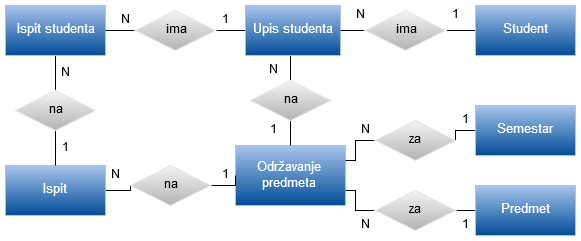
\includegraphics[width=12cm]{ev_diagram.png}
\caption{Dijagram entiteti-veze}
\label{fig:evd}
\end{figure}

Objašnjenje entiteta iz dijagrama entiteti-veze (slika \ref{fig:evd}):
\begin{itemize}
    \item Student - osnovni podaci o studentu i jedinstveni identifikator
    \item Semestar - podaci o semestru; datum početka i kraja, je li zimski ili ljetni 
    \item Predmet - osnovni podaci o predmetu; sadrži naziv i jedinstveni identifikator
    \item Održavanje predmeta - sadrži svako održavanje predmeta po semestrima
    \item Upis studenta - predstavlja upis studenta na predmet u pojedinom semestru. Dodatno sadrži konačnu ocjenu i datum kada je ocjena upisana.
    \item Ispit - održavanje ispita; sadrži tip ispita (pismeni, usmeni ili kolokvij), datum održavanja, predmet i semestar kojem pripada
    \item Ispit studenta - pojedina prijava i/ili pristupanje studenta na ispit. Sadrži kombinaciju potrebnih podataka za sve vrste ispita: je li student pristupio ispitu, dobiveni bodovi, ocjena i komentari/pitanja na usmenom. 
\end{itemize}{}

Održavanje predmeta jedinstvena je kombinacija semestra i predmeta, tj. isti predmet se ne može održavati više puta u semestru. 

Svaki student može se upisati najviše jedanput na jedno održavanje predmeta, odnosno student može upisati pojedini predmet više puta, ali u različitim semestrima.

Ispit je potrebno definirati za točno jedno održavanje predmeta, no svaki predmet može imati više ispita u svakom od semestara u kojima je definirano održavanje.

Ispit studenta je rezultat prijave odnosno pristupanja studenta na ispit iz predmeta na kojeg je upisan. Pojedini student može pristupiti istom ispitu samo jedanput. Shodno tome ispit studenta se definira za točno jedan ispit i točno jedan upis studenta. Student može pristupiti na više različitih ispita.


\chapter{Opis rješenja}
\section{Arhitektura rješenja}
Programsko rješenje je koncipirano kao višeslojni sustav prikazan na slici \ref{fig:arh} koji se sastoji od web aplikacije, windows aplikacije, sloja poslovne logike i sloja za komunikaciju s bazom podataka. Za izradu aplikacija koristi se programski okvir .NET Core i obrazac MVVM.

\begin{figure}[htb]
\centering
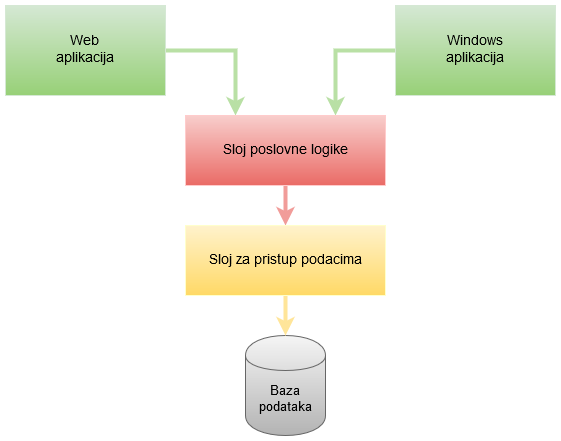
\includegraphics[width=12cm]{arh.png}
\caption{Arhitektura sustava}
\label{fig:arh}
\end{figure}

\subsection{Baza podataka i sloj za pristup podacima}
Za perzistenciju podataka korištena je relacijska baza podataka, uz poslužitelj Microsoft SQL Server.
Sloj za pristup podacima izrađen je u .NET Core-u te za pretvorbu tablica i podataka baze u klase i objekte aplikacije koristi objektno relacijski maper Entity Framework Core. 
Sustav komunicira s bazom podataka putem dane adrese \engl{connection string} te se tako postiže modularnost sustava, jer se baza podataka može zamijeniti prosljeđivanjem adrese nove baze (uz uvjet da se u novoj bazi definiraju potrebne tablice).

Sloj za pristup podacima nije ovisan ni o jednom drugom sloju, a prema van pruža sučelje za pristup podacima baze koristeći objekte .NET-a. 

\begin{figure}[htb]
\centering
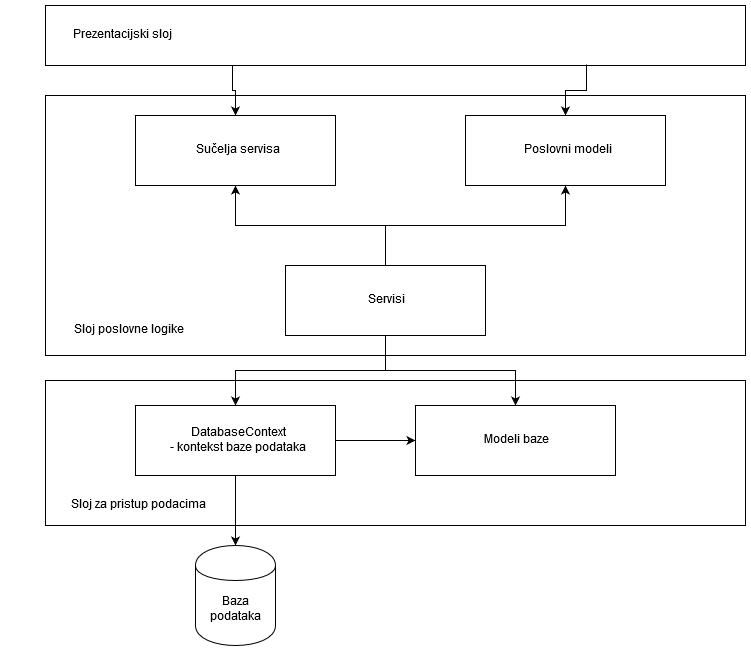
\includegraphics[width=12cm]{arhbig2.png}
\caption{Arhitektura sloja za pristup podacima i sloja poslovne logike}
\label{fig:arhbig}
\end{figure}

\subsection{Sloj poslovne logike}
Sloj poslovne logike ovisan je o sloju za pristup podacima. Obavlja pretvorbu modela baze u poslovne modele putem definiranih servisa. Pruža sučelja za pristup servisima u svrhu dohvata, spremanja ili promjene podataka.
Na slici \ref{fig:arhbig} su prikazane pojedine komponente sloja za pristup podacima i sloja poslovne logike. Također prikazane su i međusobne ovisnosti komponenata putem usmjerenih strelica.

\subsection{Prezentacijski sloj; Web i Windows aplikacija}
Web aplikacija je izrađena koristeći DotVVM programski okvir.
DotVVM je programski okvir otvorenog koda za ASP.NET Core i OWIN, a implementira obrazac MVVM.

Za izradu Windows aplikacije izabran je programski okvir Windows Presentation Foundation (u nastavku rada WPF) i .NET Core 3.0 Preview 9.
WPF je programski okvir za kreirannje korisničkih sučelja u Windows aplikacijama. Kreiran je tako da je moguće iskoristiti sve prednosti MVVM obrasca.

Programski kod u obje aplikacije podijeljen je na tri sloja: prezentacijski \engl{View}, prezentacijska logika \engl{ViewModel} i podatkovni  \engl{Model}.
 
Prezentacijski sloj direktno \engl{compile time} ovisi samo o poslovnom sloju, jer koristi poslovne modele i poziva metode sučelja servisa za obavljanje dohvata i perzistencije podataka iz prezentacijskog sloja.


\section{Podatkovni model}
Dizajn modela podataka kreiran je s idejom da se spremaju jednostavni podaci bez redundancije, a sva potrebna spajanja i kombinacije za izvršavanje zahtjeva iz prezentacijskog sloja delegirane su sloju za pristup podacima i sloja poslovne logike. Dodatno manipulacijom prikaza podataka na korisniku prihvatljiv način bavi se prezentacijski sloj.

Dizajn tablica baze (slika \ref{fig:baza}) vođen je definiranim elementima iz konceptualnog modela opisanog u poglavlju \ref{konceptualni_model}.

Dijagram baze podataka prikazan je na slici \ref{fig:baza}. Prikazani su primarni ključevi u tablicama i strani ključevi kao 1-N veze između tablica.
\begin{figure}[htb]
\centering
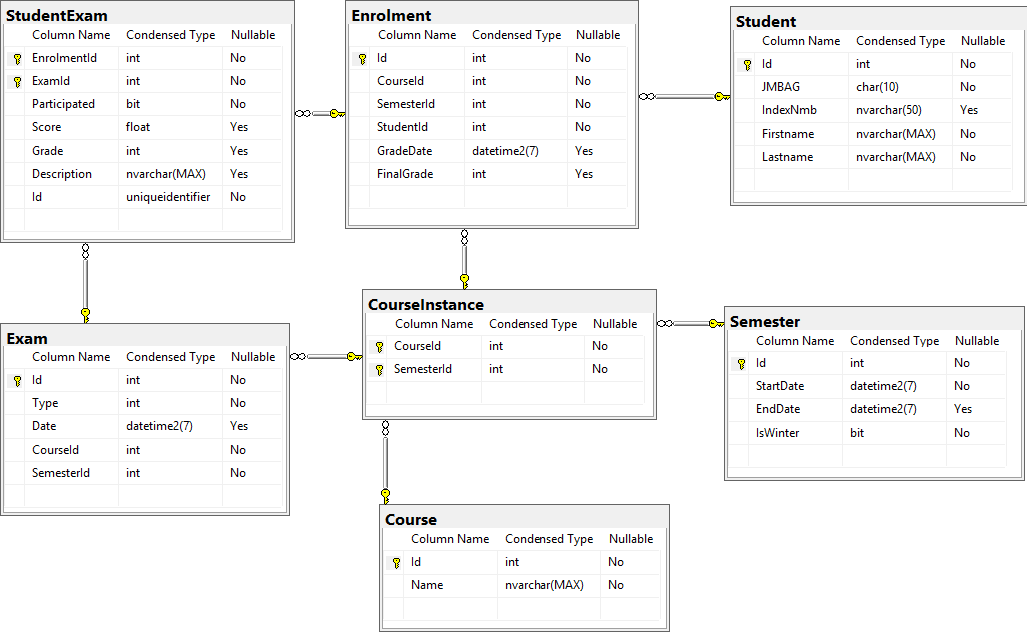
\includegraphics[width=12cm]{database_diagram3.png}
\caption{Dijagram baze podataka}
\label{fig:baza}
\end{figure}

Objašnjenje tablica:
\begin{itemize}
    \item Student - podaci o studentu: ime, prezime, JMBAG i Index
    \item Semester - podaci o semestru: datum početka i kraja, je li zimski ili ljetni semestar
    \item Course - podaci o predmetu: naziv i jedinstveni identifikator 
    \item CourseInstance - sadrži strane ključeve tablica Course i Semester. Predstavlja održavanje predmeta.
    \item Enrolment - podaci o upisu studenta na predmet u pojedinom semestru: završna ocjena i datum ocjene
    \item Exam - podaci o ispitu: tip ispita, datum održavanja, veza na održavanje predmeta
    \item StudentExam - podaci o prijavi i/ili pristupanju studenta na ispit: je li student pristupio ispitu, dobiveni bodovi, ocjena i komentari.
\end{itemize}{}

\section{Korištena tehnologija}
\subsection{Obrazac MVVM}

Model-Pogled-Prezentacijski pogled (MVVM) je arhitekturni obrazac u programiranju prikazan na slici \ref{fig:mvvm}. Olakšava odvajanje razvoja korisničkog sučelja od razvoja poslovne logike ili pozadinskog (podatkovnog) sloja. Razvijen je kako bi se olakšao razvoj korisničkih sučelja vođenih događajima \engl{event-driven}. 

Prezentacijski pogled je pretvarač vrijednosti, što znači da je odgovoran za izlaganje (pretvaranje) podatkovnih objekata iz modela na takav način da se objekti lako prezentiraju i pretvaraju. \citep{mvvm}

\begin{figure}[htb]
\centering
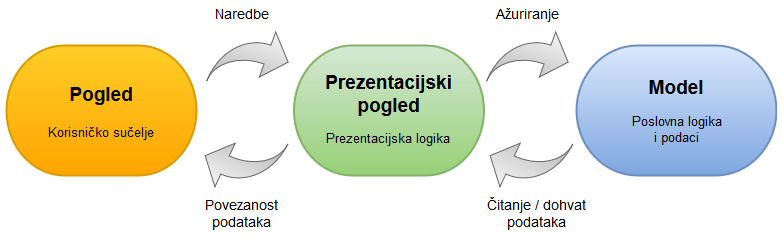
\includegraphics[width=14cm]{mvvm.png}
\caption{Arhitektura obrasca MVVM}
\label{fig:mvvm}
\end{figure}


\textbf{Model}

Model je objekt domene. Predstavlja stvarne podatke i/ili informacije. Ima odgovornost da formatira tekst ili da dohvati listu podataka. Tipično se poslovna logika drži odvojeno od modela, no zbog raznih zahtjeva u praksi se dodaju validacije i identifikatori kako bi se model mogao pratiti kroz sustav. \citep{mvvm}


\hfill\break
\textbf{Pogled}

Pogled je prezentacija podataka, ono s čime korisnik interagira(komunicira). 
Prihvaća korisnički unos i delegira upravljanje Prezentacijskom pogledu putem povezanosti podataka \engl{data-bindings}, što u konačnici manipulira vrijednostima modela.
Pogled u MVVM obrascu je aktivan, što znači da sadrži ponašanja, akcije i povezivost podataka \engl{data-bindings} te ima saznanja o Modelu i Prezentacijskom pogledu.

Bitna stvar za Pogled je da on nije odgovoran za održavanje svojeg stanja, već ga sinkronizira s Prezentacijskim pogledom. \citep{mvvm}


\hfill\break
\textbf{Prezentacijski pogled}

Prezentacijski pogled uvodi odjeljivanje modela od pogleda. Na ovaj način Model samo sadrži podatke i ne treba znati kako ih je potrebno prikazati korisniku. O prikazu podataka brine se Pogled. Prezentacijski pogled služi kao veza između Modela i Pogleda. Izlaže metode i naredbe koje pomažu održavanju stanja Pogleda, manipulaciji Modela kao rezultat akcija na Pogledu i pokreće događaje na samom Pogledu. \citep{mvvm}

\subsection{Programski okvir DotVVM}
DotVVM je programski okvir za ASP.NET Core ("Dot" iz naziva), a implementira obrazac MVVM ("VVM" iz naziva).

\begin{figure}[htb]
\centering
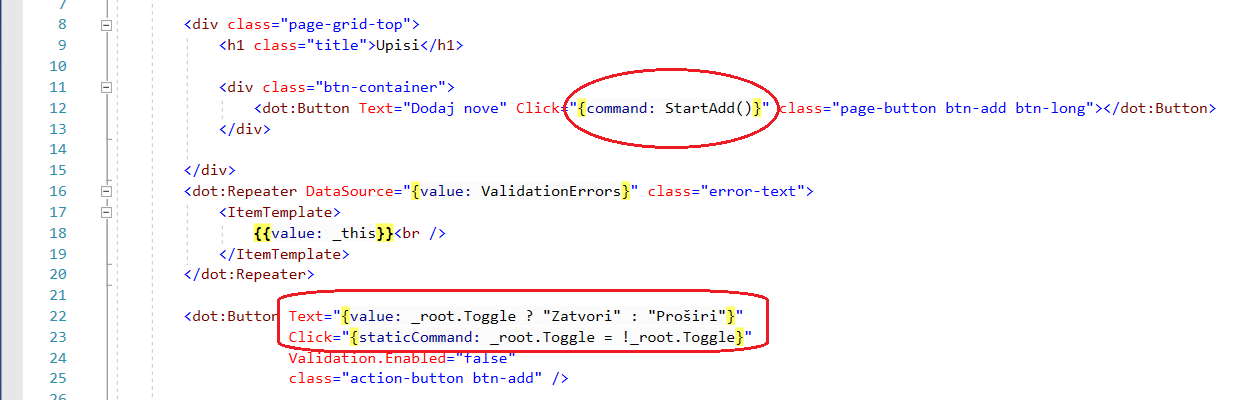
\includegraphics[width=12cm]{code_dothtml3.PNG}
\caption{Povezivanje podataka u .dothtml datoteci}
\label{fig:binding}
\end{figure}

Svaka stranica se sastoji od dvije datoteke:
\hfill\break
\hfill\break
\textbf{Pogled \engl{View}} \hfill\break
Datoteka s .dothtml ekstenzijom koja koristi obični HTML uz dodatke:
\begin{itemize}
    \item direktive - definiraju informacije vezane za stranicu %(slika \ref{fig:direktiva})
    \item povezivanje podataka \engl{data-binding} - služe za spajanje s objektima ili metodama prezentacijskog pogleda. Na slici \ref{fig:binding} prikazani redom: povezivanje naredbe \engl{command binding}, povezivanje vrijednosti objekta \engl{value-binding} i povezivanje statičke naredbe \engl{static command binding}
    \item DotVVM kontrole - sadrže definirani HTML za prikaz i Knockout.JS koji će omogućiti povezivanje podataka s objektima aplikacije. Na slici \ref{fig:controls} prikazana je vlastita kontrola (MultiSelect) i postojeća kontrola (Button).
\end{itemize}{}


\begin{figure}[htb]
\centering
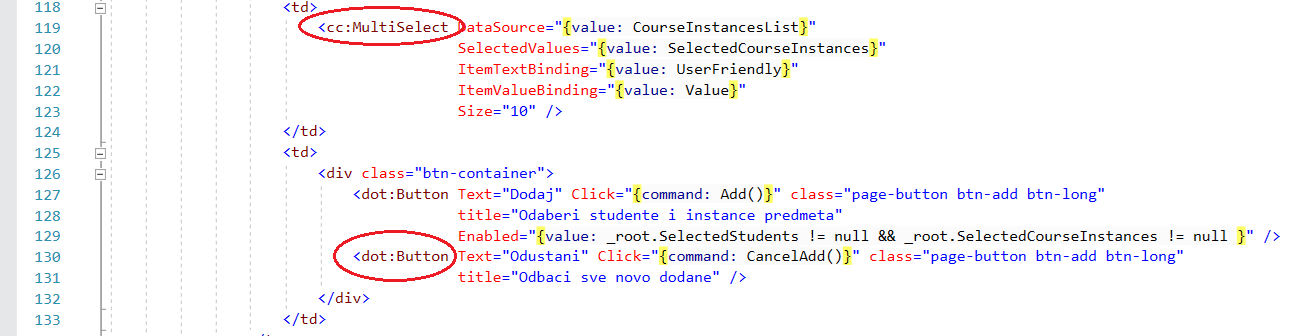
\includegraphics[width=12cm]{code_dothtml4.PNG}
\caption{DotVVM kontrole}
\label{fig:controls}
\end{figure}

\hfill\break
\textbf{Prezentacijski pogled \engl{Viewmodel}}
Obična C\# klasa koja je referencirana u .dothtml datoteci. Klasa mora biti JSON serijazibilna. Svrha joj je reprezentacija stanja stranice i definiranje naredbi koje korisnik može pokrenuti.

DotVVM ima baznu klasu za Prezentacijski pogled koja sadrži Context objekt koji omogućava interakciju s HTTP zahtjevom. 

\hfill\break
DotVVM obavlja prevođenje DotVVM kontrola u HTML, podatkovnog povezivanja \engl{data-binding} u Knockout JS izraze, povezivanja naredbi \engl{command binding} i Prezentacijskog pogleda u JavaScript.

Podatkovno povezivanje omogućava: pristup vrijednostima objekata prezentacijskog pogleda, izvršavanje njegovih metoda, izvršavanje statičkih metoda prezentacijskog pogleda ili definiranog statičkog servisa i dohvat resursa iz RESX datoteke.

Prezentacijski pogled živi na klijentu tako dugo dok je stranica učitana. Kada stranica treba pozvati metodu na serveru, prezentacijski pogled se serijalizira u JSON i šalje na server gdje će se obaviti pozvana metoda. Nastale promjene šalju se natrag na klijent. 

Ovakav način rada znači da server ne treba spremati instancu prezentacijskog pogleda u sesiji ili memoriji, ona postoji na serveru samo za vrijeme trajanja pojedinog HTTP zahtjeva. Nedostatak je što se kod poziva šalje cijeli prezentacijski pogled što može biti neefikasno.

Prezentacijski pogled u DotVVM-u ima baznu klasu "DotvvmViewModelBase" koja definira "Context" putem kojeg je moguće pristupiti podacima HTTP zahtjeva koji se obavlja i virtualne metode Init, Load i PreRender. Navedene metode imaju baznu implementaciju, ali ih je moguće nadjačati. 

Nadjačavanje Init metode obavlja se kad je potrebno obaviti dodatne radnje prije deserijalizacije podataka iz prezentacijskog pogleda. Nadjačavanje Load metode kada je potrebno obaviti dodatne radnje prije nego što se izvrše naredbe iz prezentacijskog pogleda. Za sve ostale dodatne radnje o čijim rezultatima ne ovise podaci ili metode dovoljno je nadjačati PreRender metodu.

Na slici \ref{fig:methods} je prikazan redoslijed poziva opisanih metoda i dodatne međuradnje s obzirom na radi li se o prvom učitavanju stranice ili o učitavanju stranice nakon što se pozvala neka od metoda vezana na prezentacijski pogled.

\begin{figure}[htb]
\centering
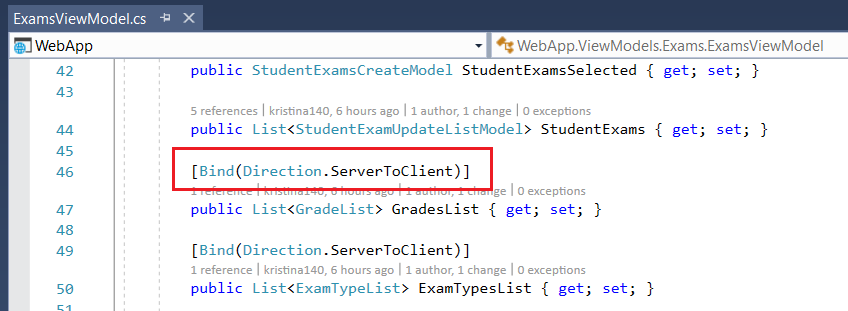
\includegraphics[width=12cm]{code_viewmodel.PNG}
\caption{Definiranje smjera slanja objekta samo sa servera na klijent}
\label{fig:bind_direction}
\end{figure}

Kao djelomično rješenje neefikasnog slanja cijelog prezentacijskog pogleda, postoje svojstva koja se mogu definirati koja će odrediti u kojem smjeru (server-klijent) se šalje objekt (slika \ref{fig:bind_direction}), za svaki objekt u prezentacijskom pogledu.



\begin{figure}[htb]
\centering
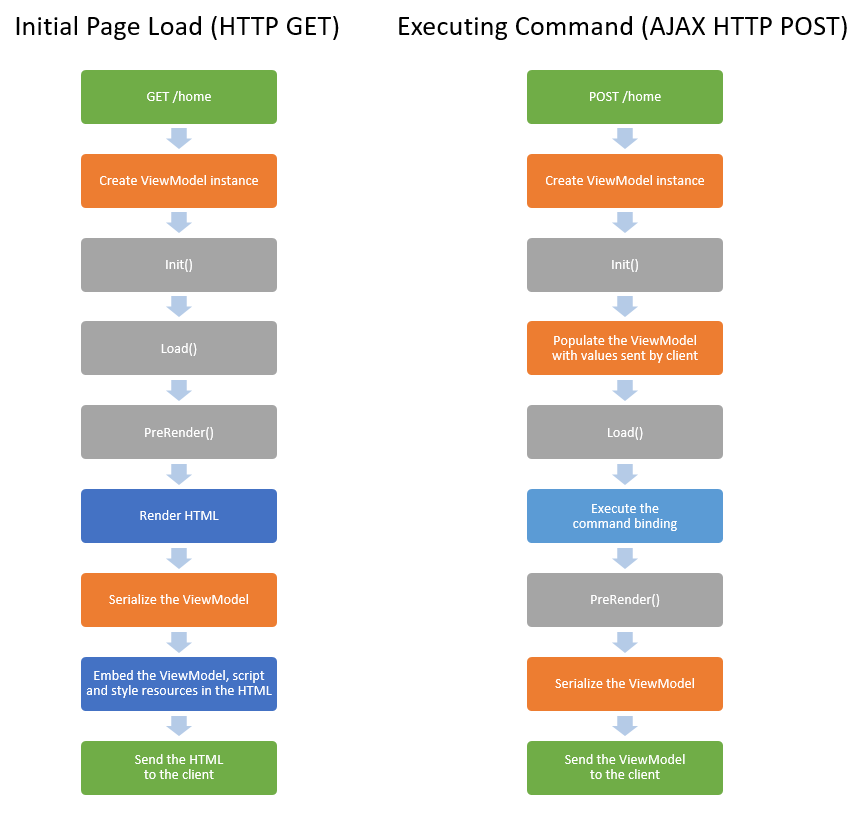
\includegraphics[width=14cm]{methods.png}
\caption{Redoslijed poziva metoda za početno učitavanje stranice i ponovno učitavanje nakon izvršenja naredbe}
\label{fig:methods}
\end{figure}


\subsection{Programski okvir .NET Core}

.NET Core je besplatan programski okvir otvorenog koda \engl{open-source} za operacijske sustave Windows, Linux i MacOS. Razvio ga je Microsoft kao nasljednika za .NET Framework. Služi za izgradnju modernih, oblak baziranih \engl{cloud-based} i internetom povezanih aplikacija. \citep{dotnet}

U usporedbi sa starim .NET Frameworkom neka od poboljšanja su:
\begin{itemize}
    \item ujedinjenje ASP.NET MVC (model - pogled - kontroler) i ASP.NET Web API (programski okvir za izgradnju HTTP servisa za web preglednike i mobilne uređaje) u jedinstveni programski model
    \item podrška za tip verzioniranja gdje različite aplikacije koje se vrte na istoj mašini mogu ciljati različite verzije ASP.NET Core-a
\end{itemize}{}


\hfill\break
\textbf{.NET Core 3.0 (Preview)}

Nova verzija .NET Cora uvela je podršku za Windows aplikacije, točnije za Windows Forms i Windows Presentation Foundation (WPF) aplikacije, ali trenutno samo za Windows platformu.

Za izgradnju lako nadogradivih aplikacija čiji dijelovi su što više neovisni te jednostavno zamjenjivi, koristi se ubacivanje ovisnosti \engl{Dependency Injection} (nadalje DI). DI je tehnika inverzije \engl{Inversion of Control} kontrole u kojoj jedan objekt osigurava odnosno predaje ovisnosti o kojima ovisi drugi objekt. 

.NET Core pruža ugrađenu potporu za DI, a najčešće se koristi u ASP.NET Core aplikacijama. Primjer je Startup.cs datoteka u web aplikaciji ovog rada. Ona sadrži metodu ConfigureServices u kojoj se definiraju servisi koji će se dodati u interni kontejner kojeg onda .NET Core koristi kako bi obavio DI. Opisana metoda poziva se kod pokretanja aplikacije.

Prema definiranoj arhitekturi sustava, Windows aplikacija i web aplikacija koriste zajednički poslovni sloj za obavljanje poslovne logike i perzistencije podataka. U poslovnom sloju definirani su servisi koji obavljaju logiku sustava, a kojima se pristupa putem definiranih sučelja. Za web aplikaciju korišteni su ASP.NET IOC kontejneri iz paketa Microsoft Extensions DependecyInjection kako bi se u prezentacijski sloj ubacili potrebni servisi. 
Zbog korištenja nove verzije .NET Core-a, navedene pakete bilo je moguće uključiti i u Windows aplikaciju. 

Ulazna točka WPF aplikacije je "main" metoda koja se nalazi u datoteci App.xaml.cs. Iz naslijeđene klase (Application) nadjačava se metoda OnStartup, koja se poziva kod pokretanja aplikacije, te se u njoj definira i konfigurira DI kontejner i servisi. Definiranje DI nastavlja se u metodi ConfigureServices na jednak način kao u web aplikaciji. Dodatno, registrira se početni prozor aplikacije kako bi i njega ubacili u DI lanac. Slika \ref{fig:app_DI} prikazuje isječak koda koji obavlja opisanu funkcionalnost.

\begin{figure}[htb]
\centering
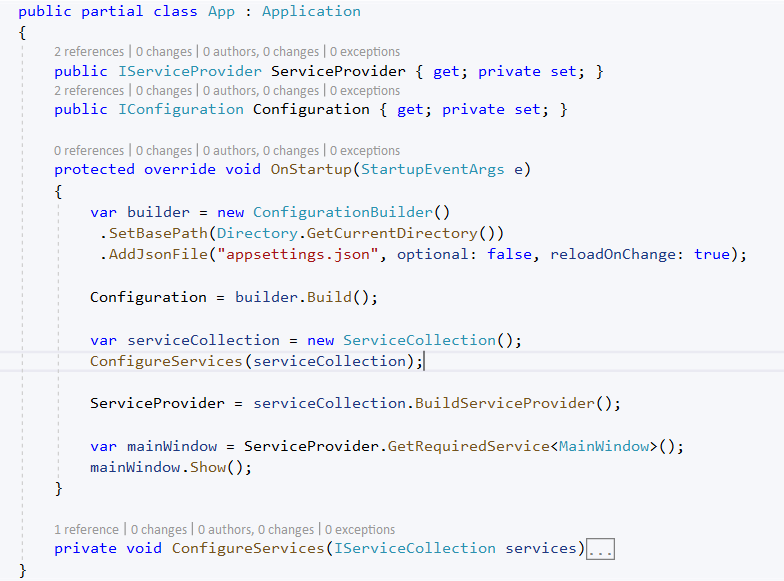
\includegraphics[width=14cm]{code_app_DI.PNG}
\caption{Defiranje ASP.NET IOC kontejnera za DI u WPF aplikaciji }
\label{fig:app_DI}
\end{figure}


\subsection{Windows Presentation Foundation}
WPF je programski okvir za kreiranje korisničkih sučelja u Windows aplikacijama. Podskup je .NET tipova koji se nalaze u  "System.Windows" imenskom prostoru. Uključuje dodatne programske konstrukte koji poboljšavaju svojstva \engl{properties} i događaje \engl{events} : "dependency properties" i "routed events".

Svrha ovisnih svojstava \engl{dependency properties} je pružanje načina izračuna vrijednosti svojstva temeljenih na vrijednostima drugih ulaza. Drugi ulazi mogu biti sistemska svojstva, mehanizam određivanja svojstva (točno-na-vrijeme) poput vezanja podataka \engl{data binding}, predlošci za višestruku uporabu ili vrijednosti putem roditelj-dijete veze s ostalim elementima u stablu elemenata.
Dodatno navedena svojstva mogu implementirati samostalnu validaciju, zadanu vrijednost, pozive koji promatraju promjene na drugim svojstvima. \citep{wpf}

Preusmjereni događaj \engl{routed event} je vrsta događaja koja može pozvati rukovatelje \engl{handler} na više slušatelja u stablu elemenata, a ne samo na objekt koji je podigao događaj. 

WPF omogućava izradu aplikacije koristeći XAML ili "kod iza" (C\#) za definiranje izgleda i popratne logike koja odgovara na korisničku interakciju.

WPF podržava vezanje podataka na jednostavan i konzistentan način. Elementi se mogu vezati na podatke iz različitih izvora. Različite kontrole (prikaz podataka) podržavaju fleksibilno sliliziranje kod prikaza podataka. Dodatno za nekoje kontrole moguće je definirati sortiranje, filtriranje i grupiranje nad podacima.

Mogućnost vezanja podataka je ono što omogućava upotrebu MVVM obrasca. Vezanja se definiraju u Pogledu i vezuju podatke na Prezentacijskom pogledu.

Kako bi se definirala veza između Prezentacijskog pogleda i prozora WPF aplikacije, WPF koristi DataContext svojstvo. Svakom elementu korisničkog sučelja moguće je definirati DataContext. Ako se nekom od elemenata ne definira kontekst podataka tada ga on nasljeđuje od roditelja. Stoga, postavljanjem DataContexta na prozor efektivno se postavlja i na svaki element korisničkog sučelja.

Kako bi se obavilo javljanje Pogledu da je došlo do promjena na izvoru podataka (Prezentacijski pogled) potrebno je implementirati  INotifyPropertyChanged (INPC) sučelje u Prezentacijski pogled i Model. Svaki put kada se svojstvo promjeni podigne se događaj koji će Pogled uhvatiti i zatim osvježiti podatke.

\begin{figure}[htb]
\centering
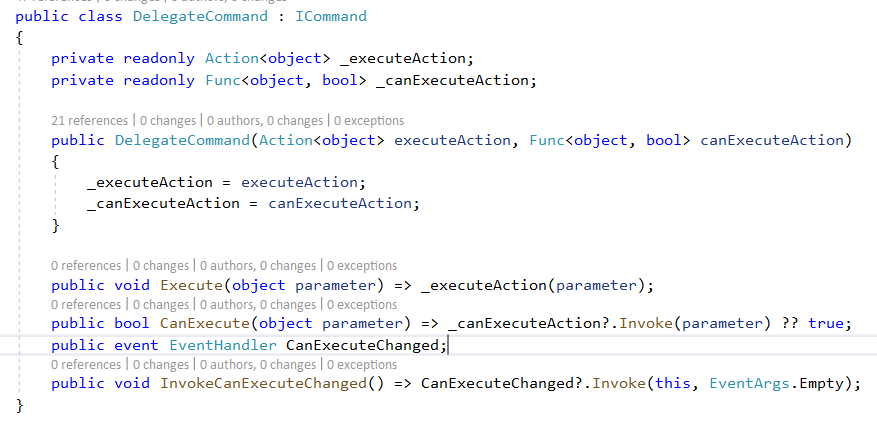
\includegraphics[width=14cm]{delegatecommand.PNG}
\caption{Isječak koda koji prikazuje implementaciju korisničke naredbe pogodne za MVVM obrazac}
\label{fig:delegatecommand}
\end{figure}

WPF omogućava kreiranje naredbi \engl{Commands}. One služe tome da se poruke prenose s Pogleda na Prezentacijski pogled vođenih korisničkom interakcijom (pr. pritisak gumba). WPF interno ne podržava idealni način za kreiranje korisničkih naredbi za Prezentacijski pogled u sklopu MVVM obrasca pa je na slici \ref{fig:delegatecommand} dana potrebna implementacija. Definira se akcija koja će se obaviti kada se naredba pozove i način provjere može li se naredba trenutno obaviti.

\subsection{EPPlus}
EPPlus je .NET biblioteka koja omogućava čitanje i kreiranje Excel datoteka koristeći Office Open XML format (xlsx). 

Korišten za izradu izvješća, a odabran je jer se izvješća kreiraju na serveru. Takav način omogućava da se funkcionalnost izrade smjesti u servis na poslovnom sloju. Web i Windows aplikacija zatim servisu pristupaju preko danog sučelja. Posljedica je jednako izvješće neovisno o aplikaciji.

\chapter{Ostvarena funkcionalnost}

Sustav podržava dohvat, uređivanje i brisanje svih podataka. Podaci se prikazuju tablično ili u listama ovisno o međusobnoj povezanosti. Također sustav podržava i izvoz podataka u Microsoft Excel. Aplikacija je rađena s ciljem da bude korisnički intuitivna, da bitne akcije na stranicama budu uočljive i lako razumljive. Svi akcijski gumbi i linkovi imaju boju koja odražava tip akcije koju obavljaju, te je tako plava dohvat ili prikaz podataka, zelena je akcija spremanja, narančasta označava odbacivanje unesenih podataka i crvena da se radi o akciji brisanja. Dodatno radi zaštite od slučajnog krivog klika, svi gumbi koji obavljaju akciju brisanja najprije prikažu formu za potvrdu akcije. 

\section{Web aplikacija}

\subsection{Manipulacija osnovnim podacima}
Svrha aplikacije je vođenje evidencije o izlascima i rezultatima studenata na ispitima. Kako bi to omogućili potrebno je najprije dodati osnovne podatke na kojima će se graditi ostatak informacija koje sustav sadrži.
Iz tog razloga aplikacija pruža uslugu tabličnog prikaza svih osnovnih podataka, uređivanja podataka na mjestu, brisanja stavki i kreiranja novih. Svaka od osnovnih komponenti nalazi se na vlastitoj stranici odnosno url adresi radi bolje preglednosti. 

Zbog boljeg korisničkog iskustva i lakše navigacije u aplikaciji, stranice sadrže korisne linkove na vezane podatke, gumbe s funkcionalnošću prikaza odnosno skrivanja određenog dijela podataka, dohvata dodatnih podataka i prikaza prozora forme \engl{modal window};


\subsubsection{Predmeti}
Jedan od temeljnih podataka sustava je predmet. Aplikacija pruža tablični prikaz svih spremljenih predmeta. Uz prikaz osnovnih podataka moguće je proširiti (pritiskom na gumb Proširi slika \ref{fig:course}) prikaz s podacima o održavanju predmeta u semestrima.

\begin{figure}[htb]
\centering
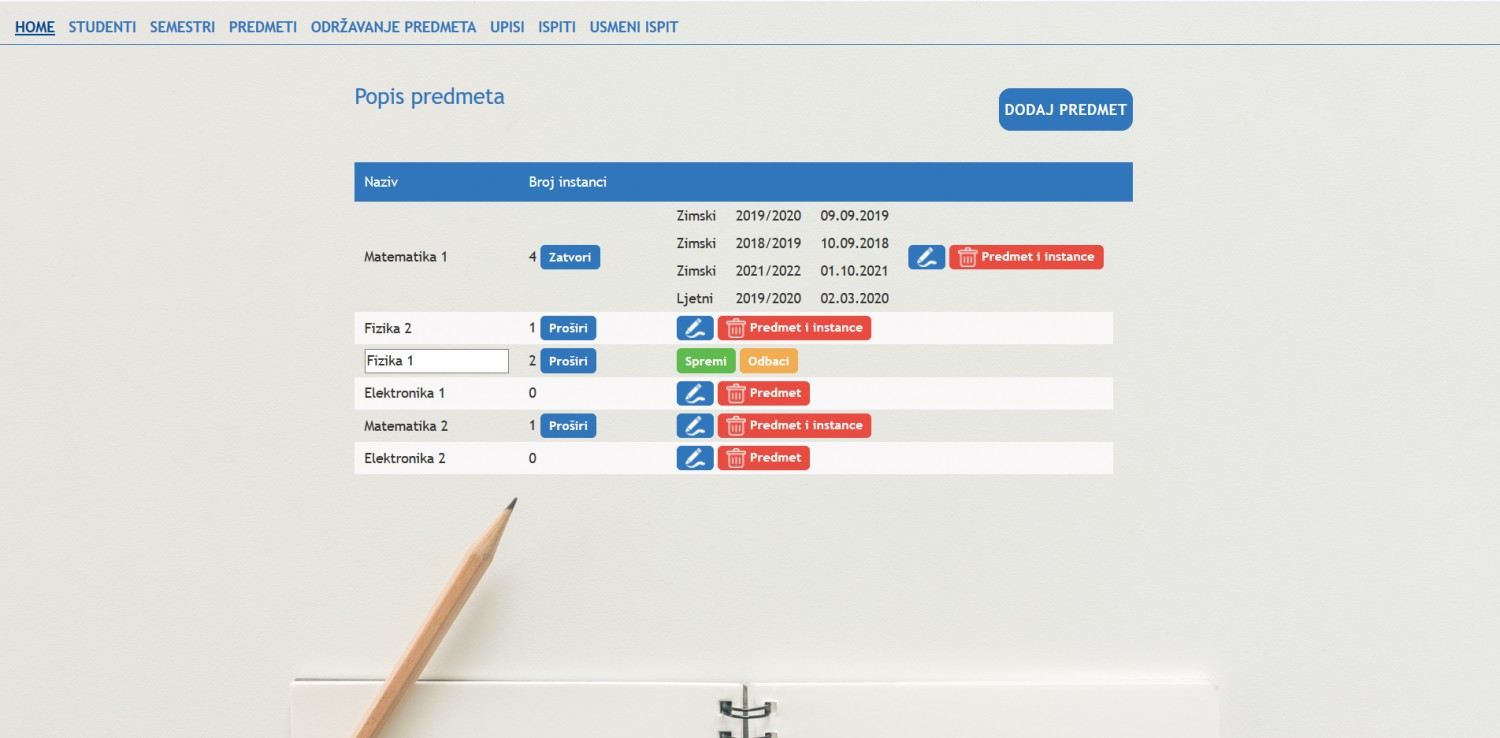
\includegraphics[width=14cm]{predmeti_edit.jpg}
\caption{Stranica web aplikacije za prikaz, uređivanje i brisanje predmeta}
\label{fig:course}
\end{figure}

Svaki prikazani predmet moguće je na mjestu urediti i spremiti promjene. Uz uređivanje dostupno je i brisanje čija akcija ovisi o postojećim podacima u bazi. Ako predmet sadrži instance odnosno održava se u nekom semestru, tada će se brisanjem predmeta obrisati i sve instance održavanja predmeta, inače se briše samo predmet. Vrsta akcije naznačena je na gumbu za brisanje (slika \ref{fig:course}). 

Akcija kreiranja novog predmeta pokreće se pritiskom na gumb "DODAJ PREDMET" koji otvara formu za unos potrebnih podataka te nudi opciju spremanja ili odustajanja od akcije.

\begin{figure}[htb]
\centering
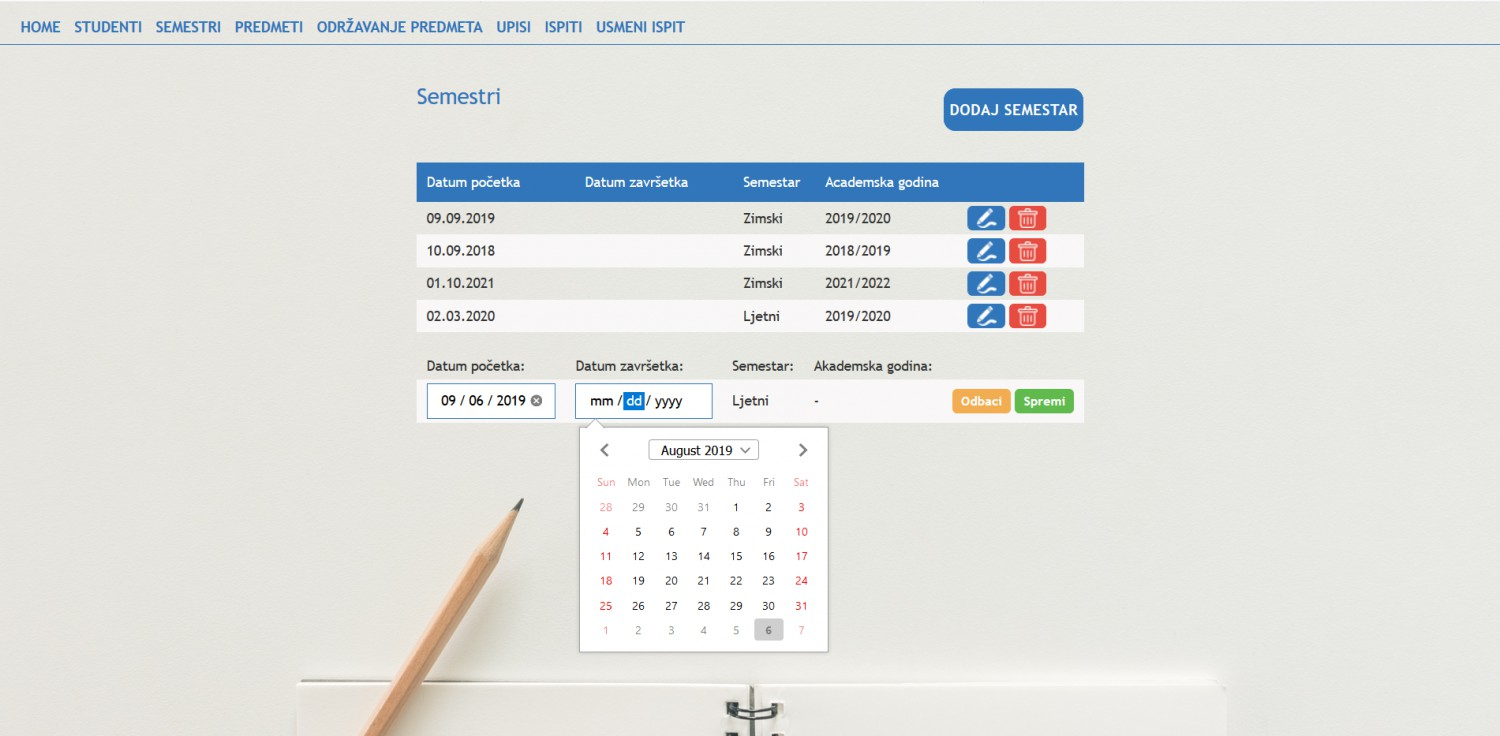
\includegraphics[width=14cm]{semestri_add.jpg}
\caption{Stranica web aplikacije za prikaz, uređivanje i brisanje semestara}
\label{fig:semester}
\end{figure}

\subsubsection{Semestri} \label{semestri_section}
Kako bi mogli kreirati održavanje predmeta potrebno je najprije definirati semestre. Semestar je definiran datumom početka iz kojeg aplikacija samostalno izračunava akademsku godinu i radi li se o zimskom ili ljetnom semestru (programski isječak na slici \ref{fig:semester_type}). Opcionalno moguće je definirati i datum završetka semestra. Prikaz stranice na slici \ref{fig:semester}.

\begin{figure}[htb]
\centering
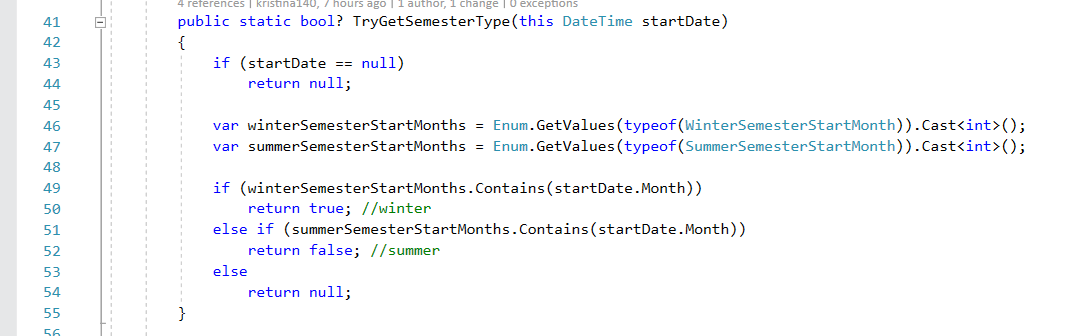
\includegraphics[width=14cm]{code_semester.PNG}
\caption{Programski isječak za određivanje vrste semestra}
\label{fig:semester_type}
\end{figure}

Za kreiranje semestra sustav podržava samo određene mjesece koji se smatraju važećima. Po unosu nevažećeg mjeseca sustav će obavijestiti korisnika i ispisati koji mjeseci su valjani. Programski isječak na slici \ref{fig:semester_call} prikazuje poziv metode za određivanje semestra odmah po unosu datuma. Ovakvo ograničenje omogućava automatizirano određivanje vrste semestra.

\begin{figure}[htb]
\centering
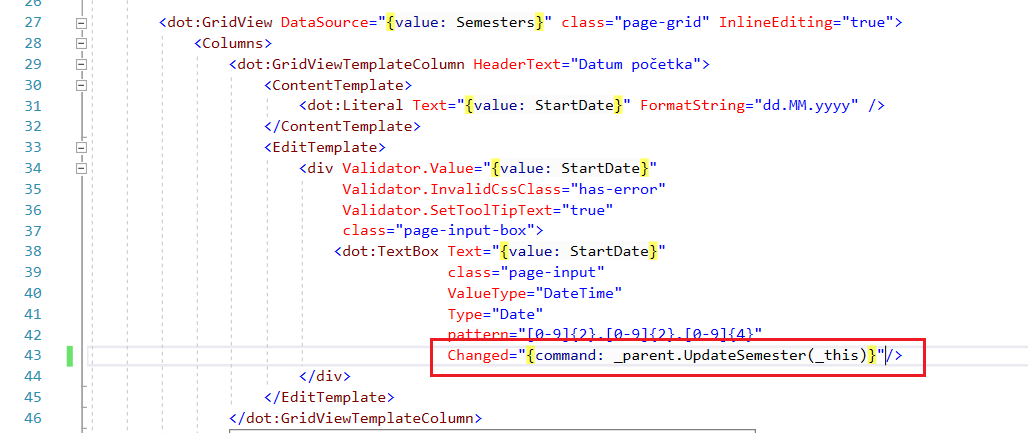
\includegraphics[width=14cm]{code_semester2.PNG}
\caption{Programski isječak za poziv metode za izračun semestra i akademske godine odmah po unosu datuma }
\label{fig:semester_call}
\end{figure}

\subsubsection{Studenti}
Posljednja osnovna stavka aplikacije su studenti. Prikazuju se u tabličnom obliku na vlastitoj stranici (slika \ref{fig:student}). Moguće je na mjestu urediti podatke i obrisati studenta. 

\begin{figure}[htb]
\centering
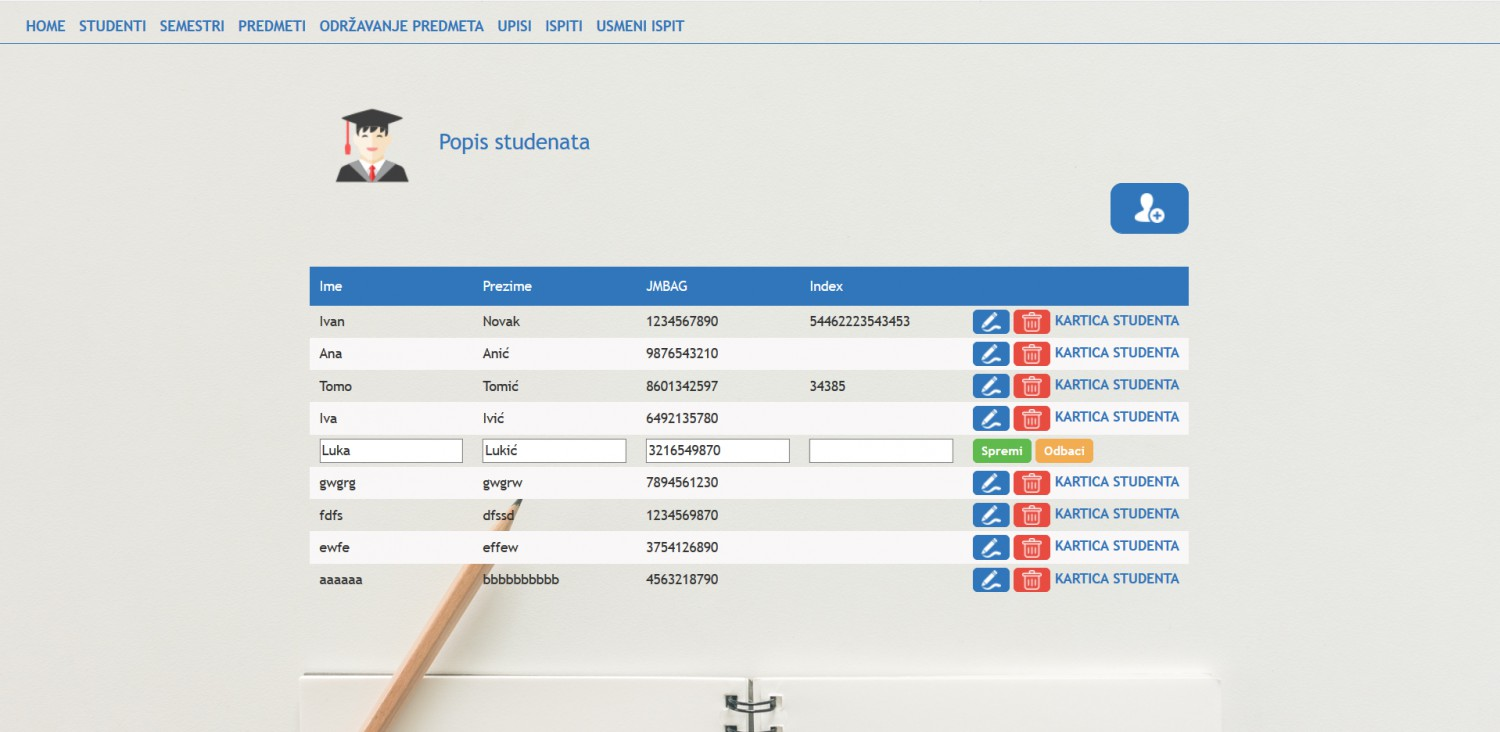
\includegraphics[width=14cm]{studenti_edit.jpg}
\caption{Stranica web aplikacije za prikaz, uređivanje i brisanje studenata }
\label{fig:student}
\end{figure}

Kod dodavanja novog studenta obavezno je navesti ime, prezime i JMBAG.

\begin{figure}[htb]
\centering
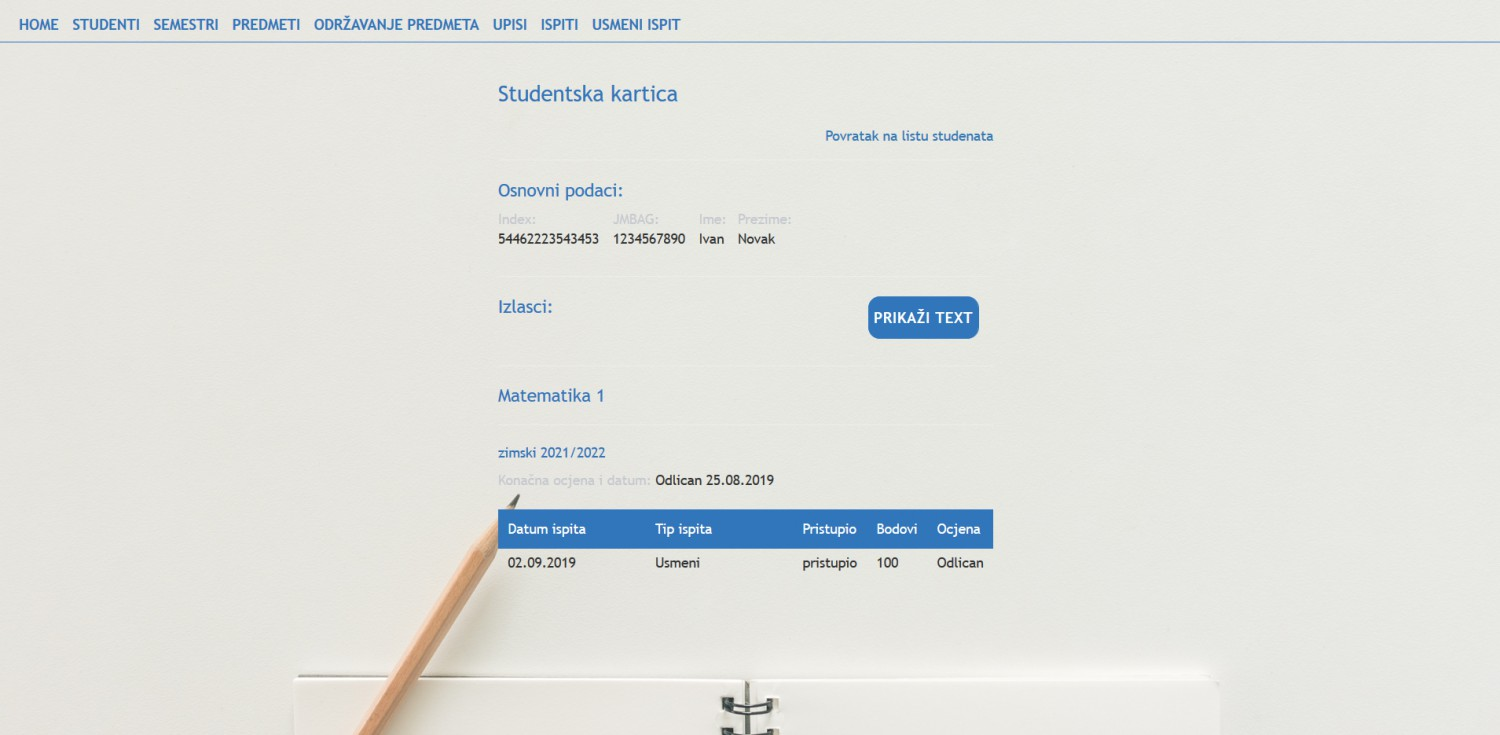
\includegraphics[width=14cm]{studentska_kartica.jpg}
\caption{Stranica web aplikacije za pregled svih aktivnosti studenta }
\label{fig:kartica}
\end{figure}

Dodatna funkcionalnost je dohvat svih podataka o studentu, u što spadaju osnovni podaci i prisustvovanje na ispitima te rezultati s istih (slika \ref{fig:kartica}). Podaci su grupirani najprije po predmetima a zatim po semestrima. Za svaki par predmet i semestar ispisuje se konačna ocjena i datum ocjene ako je ista ostvarena. Za svaki od ispita u semestru ispisuje se tablica sa svim osnovnim podacima iz ispita.
Navedena funkcionalnost dostupna je putem linka "KARTICA STUDENTA" koji se nalazi uz svakog od studenata.

\subsection{Održavanje predmeta i upisi studenata}

\subsubsection{Održavanje predmeta}
Dodatna stranica koja tablično prikazuje sve instance predmeta (slika \ref{fig:instance}). Instanca predmeta se sastoji od spajanja predmeta i semestra, i kao takva nema podataka za uređivanje te ju je moguće samo obrisati. Aplikacija pruža korisnički jednostavan način brisanja samo instance ili brisanja i vezanog predmeta za svim njegovim instancama, ponudom dva gumba čiji opisi objašnjavaju vrstu akcije.

Kod kreiranja instance potrebno je izabrati predmet i semestar iz padajućih izbornika. Ako željeni podaci ne postoje u padajućim izbornicima ispod njih se nalazi gumb putem kojeg se otvara forma za kreiranje novog predmeta odnosno semestra.

\begin{figure}[htb]
\centering
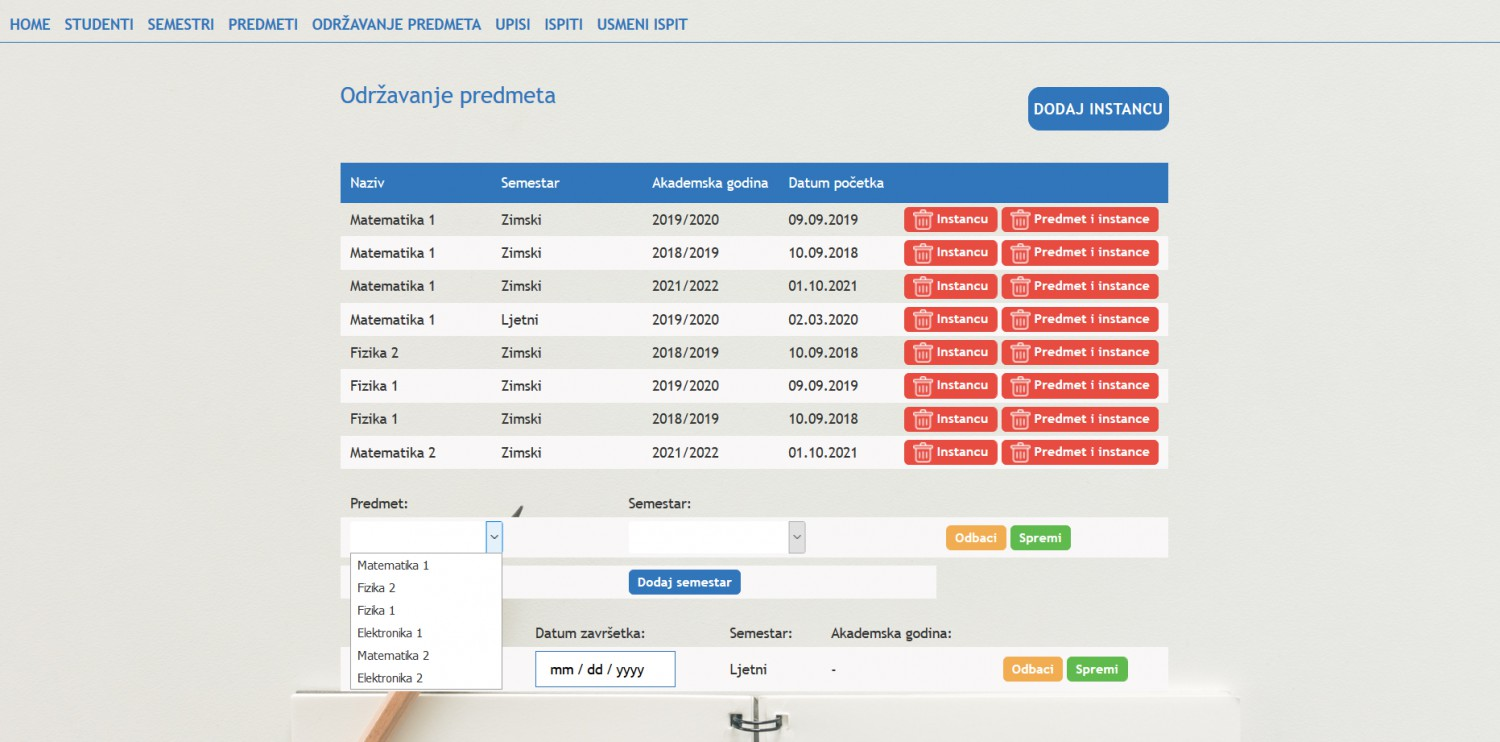
\includegraphics[width=14cm]{odrzavanja_predmeta_add.jpg}
\caption{Stranica web aplikacije za pregled i dodavanje održavanja predmeta }
\label{fig:instance}
\end{figure}

\subsubsection{Upisi studenata}
Upis studenta \engl{Enrolment} označava upisanog studenta na jednoj instanci predmeta i dodatno sadrži zaključnu ocjenu i datum ocjene. Prikaz podataka je tabličnog tipa na zasebnoj stranici (slika \ref{fig:upis}). Svaki od upisa moguće je obrisati i urediti. Uređivanje uključuje samo promjenu ocjene i datuma ocjene.

\begin{figure}[htb]
\centering
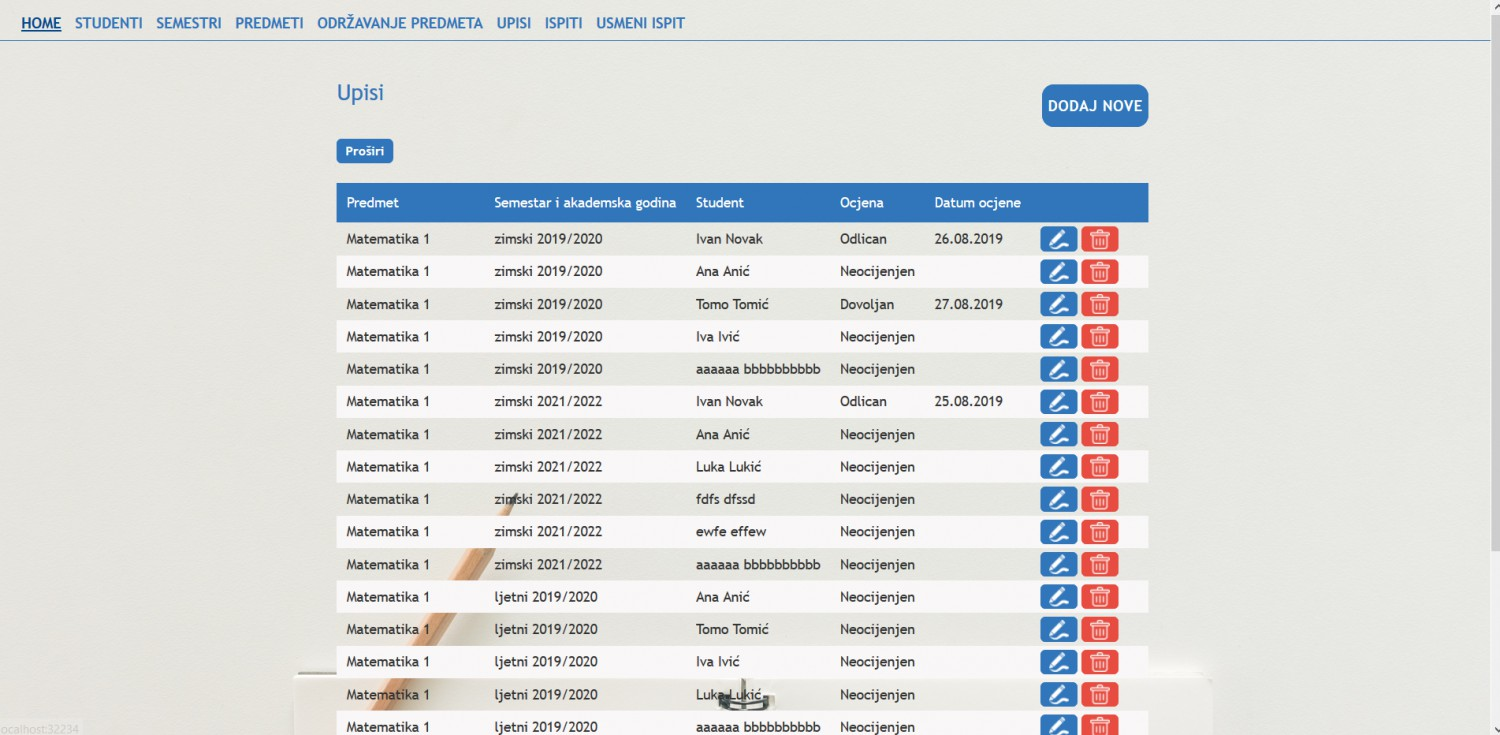
\includegraphics[width=14cm]{upisi.jpg}
\caption{Stranica web aplikacije za pregled, uređivanje i dodavanje upisa studenata na predmet }
\label{fig:upis}
\end{figure}

Dodatna akcija na stranici je gumb proširi koji će prikazati odnosno sakriti ostale podatke o studentu. Podaci su inicijalno sakriveni zbog preglednosti, ali je dana mogućnost prikaza zbog identifikacije studenata istog imena i prezimena.

Akcija "DODAJ NOVE" otvara formu (slika \ref{fig:upisi_dodaj}) koja sadrži popis studenata i popis održavanja predmeta. Iz obje liste moguće je odabrati više stavki te će se pritiskom na gumb dodaj privremeno kreirati sve kombinacije odabranih studenata i održavanja predmeta. Kreirane kombinacije prikazuju se tablično na dnu stranice gdje je dodatno omogućeno uređivanje podataka o ocjeni i datumu ocjene za svaki par. Uz uređivanje moguće je i odbaciti neke od kreiranih parova ili ponovnim izborom dodati nove.
\hfill\break

\begin{figure}[htb]
\centering
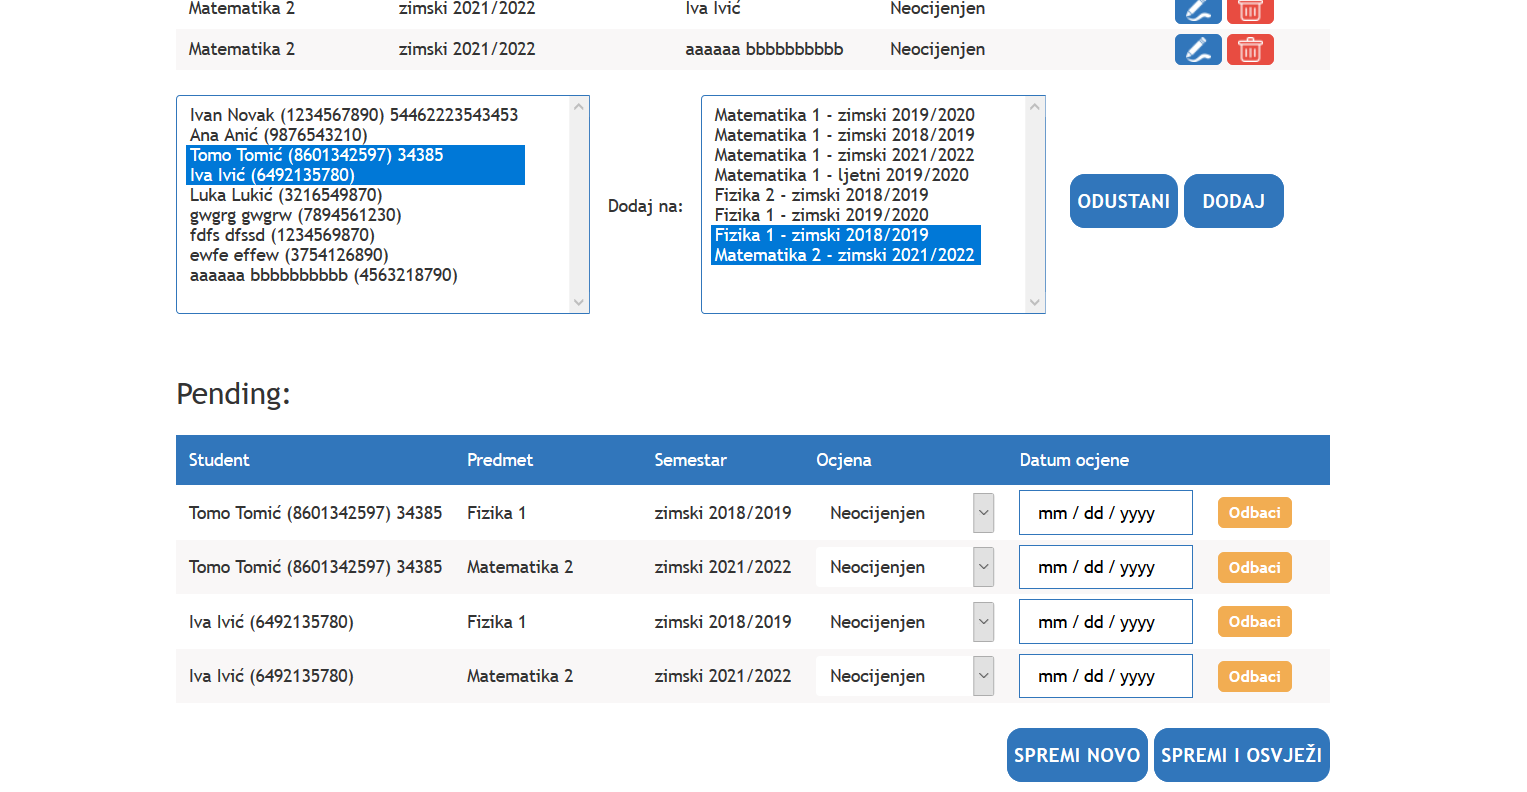
\includegraphics[width=14cm]{upisi_dodaj.PNG}
\caption{Isječak stranice upisa studenata s formom za dodavanje  }
\label{fig:upisi_dodaj}
\end{figure}

\hfill\break
Forma nudi dvije opcije spremanja privremeno kreiranih kombinacija. Prva opcija "SPREMI NOVO" će zanemariti sve postojeće kombinacije u bazi i kreirati samo nove. Druga opcija "SPREMI I OSVJEŽI" će kreirati nove, a postojećima će osvježiti novo unesene vrijednosti ocjena i datuma. Postavljanjem miša iznad pojedinog gumba prikazat će se navedeni opisi akcija.



\subsection{Ispiti}
\subsubsection{Popis svih ispita}
Stranica ispiti sadrži tablični prikaz svih postojećih ispita i vezanih podataka (slika \ref{fig:ispiti}). Odabirom opcije uredi otvaraju se polja za uređivanje datuma i vremena ispita.
Postoje dvije opcije brisanja: brisanje ispita i brisanje ispita i svih studentskih pristupanja ispitu. Sustav neće dozvoliti brisanje samo ispita, ako isti ima vezane stavke.

\begin{figure}[htb]
\centering
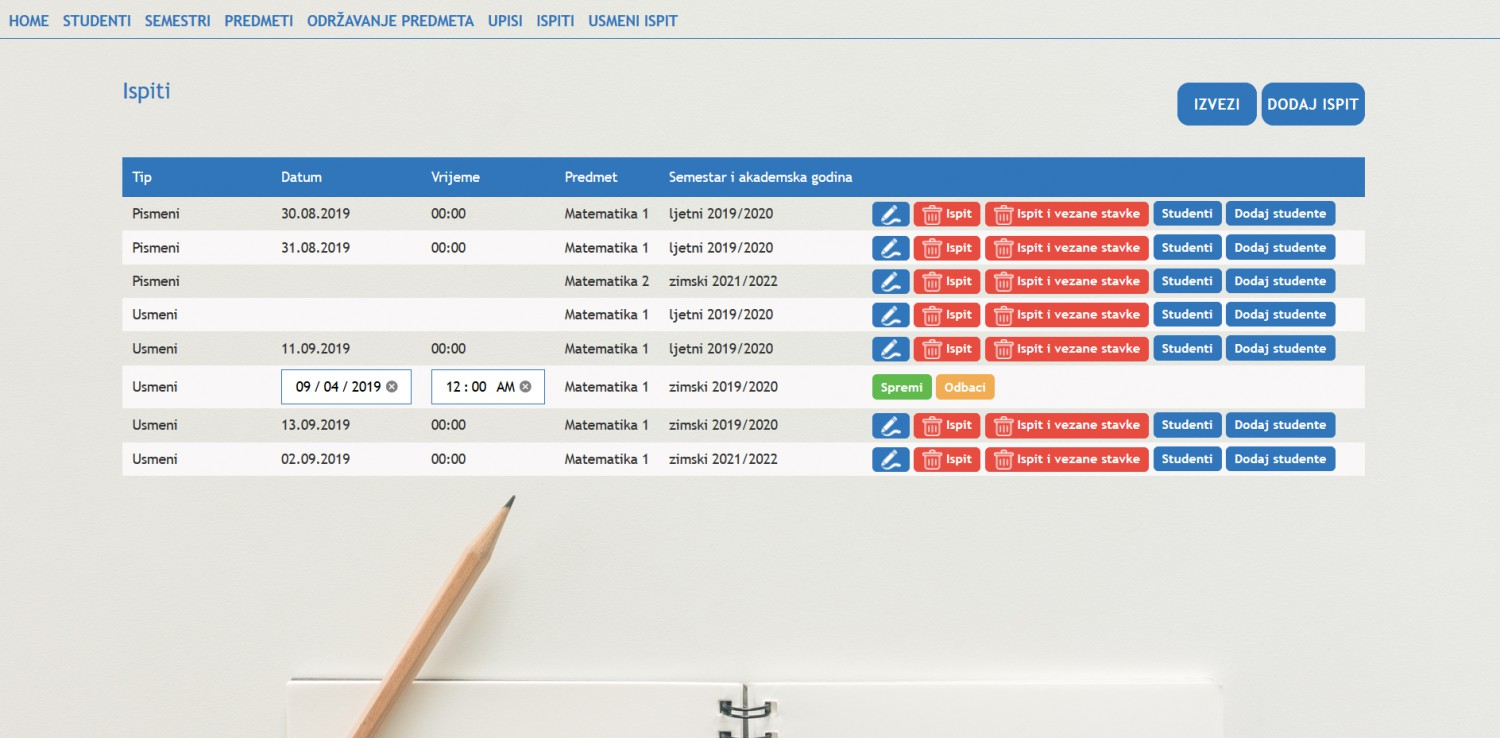
\includegraphics[width=14cm]{ispiti.jpg}
\caption{Stranica web aplikacije za pregled, uređivanje i dodavanje ispita }
\label{fig:ispiti}
\end{figure}

Akcija dodaj ispit otvara formu (slika \ref{fig:ispiti_add})  gdje je potrebno odabrati vrstu ispita i za koji predmet (točnije instancu predmeta) se održava. Nakon izbora instance predmeta dohvaćaju se svi studenti koji su upisani na taj predmet u tom semestru. Lista studenata omogućava izbor više njih. Opcionalne vrijednosti kod kreiranja ispita su datum i vrijeme ispita i upis studenata na ispit.

\begin{figure}[htb]
\centering
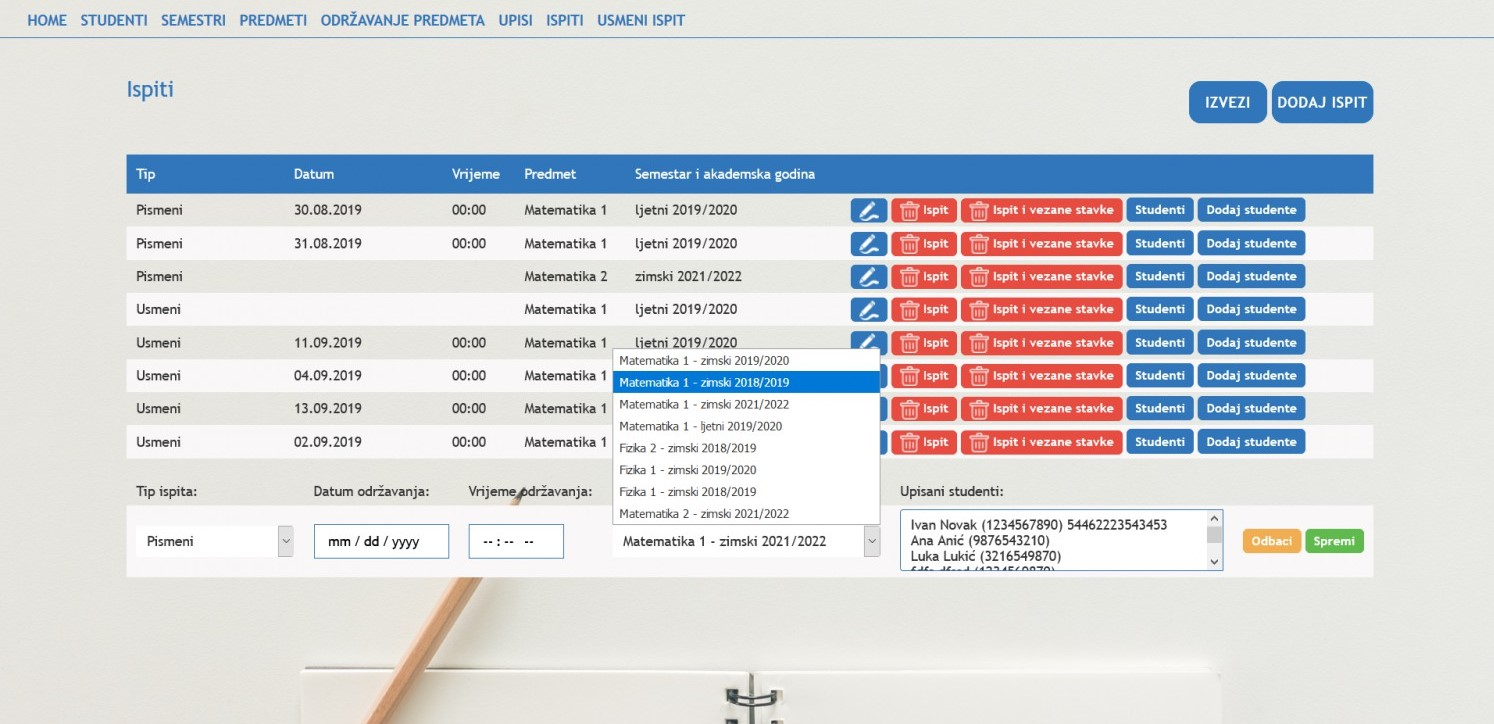
\includegraphics[width=14cm]{ispiti_addispit.jpg}
\caption{Isječak stranice ispita s formom za kreiranje novog }
\label{fig:ispiti_add}
\end{figure}

Dodatne akcije na stranici su : 
\hfill\break
\textbf{"Studenti"} \hfill\break
akcija se nalazi uz svaki ispit. Dohvaća popis svih studenata koji su upisali ispit i omogućava uređivanje podataka (je li pristupio, ocjena, datum ocjene, text pitanja), brisanje pojedinog studentskog ispita, te ako je usmeni dodatnu akciju odlaska na stranicu za detaljniji prikaz podataka za usmeni ispit. Unesene promjene moguće je zasebno spremiti (gumb za spremanje se pojavljuje nakon detektiranja promjena) ili sve zajedno na gumb "SPREMI SVE PROMJENE". Prikazano na slici \ref{fig:ispiti_studenti}.

\begin{figure}[htb]
\centering
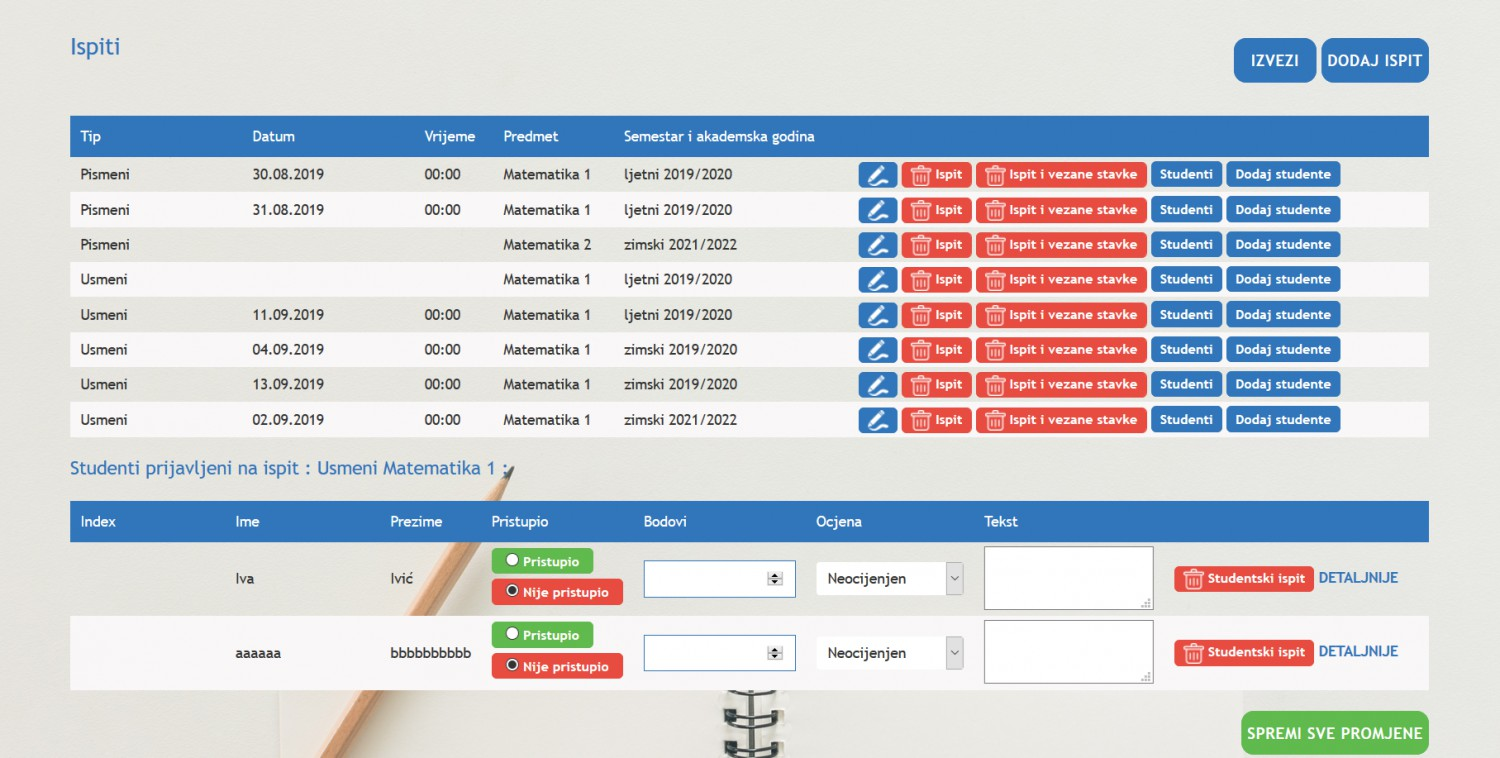
\includegraphics[width=14cm]{ispiti_studenti.jpg}
\caption{Isječak stranice ispita s prikazom studenata upisanih na ispit}
\label{fig:ispiti_studenti}
\end{figure}

\hfill\break
\textbf{"Dodaj studente"} \hfill\break
akcija se nalazi uz svaki ispit. Prikazuje formu za mogući višestruki izbor studenata koji će se upisati na ispit (slika \ref{fig:ispiti_studenti_add}). Nakon potvrde moguće je urediti podatke.

\begin{figure}[htb]
\centering
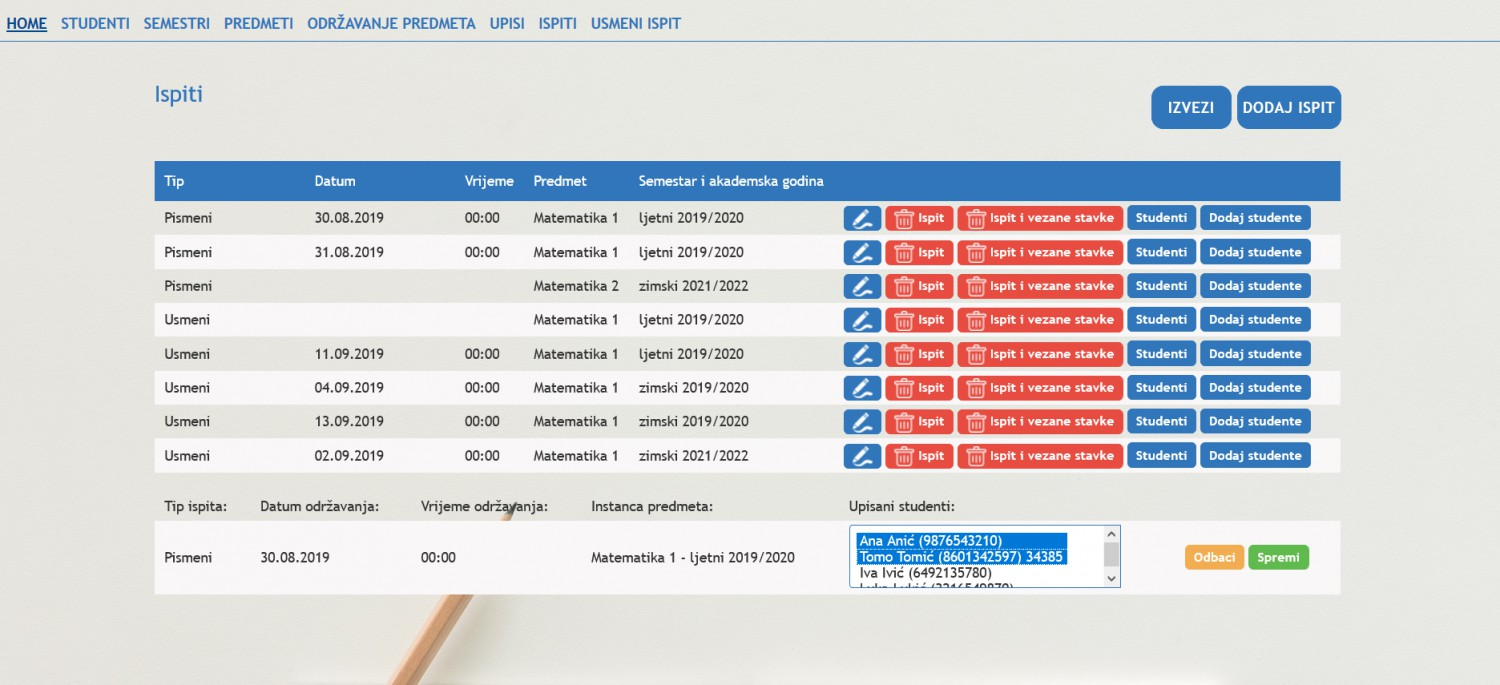
\includegraphics[width=14cm]{ispiti_addstudents.jpg}
\caption{Isječak stranice ispita s prikazom forme za dodavanje studenata na ispit}
\label{fig:ispiti_studenti_add}
\end{figure}

\hfill\break
\textbf{"Izvezi"} \hfill\break
akcija otvara formu u kojoj je potrebno odabrati predmet i semestar te opcionalno upisati naziv datoteke. Pritiskom na gumb "IZVEZI" kreira se Microsoft Excel datoteka s popisom svih studenata, ispita, prisustvovanja i ostvarenja na ispitima za dani predmet i semestar. Prikazano na slici \ref{fig:export}.


\begin{figure}[htb]
\centering
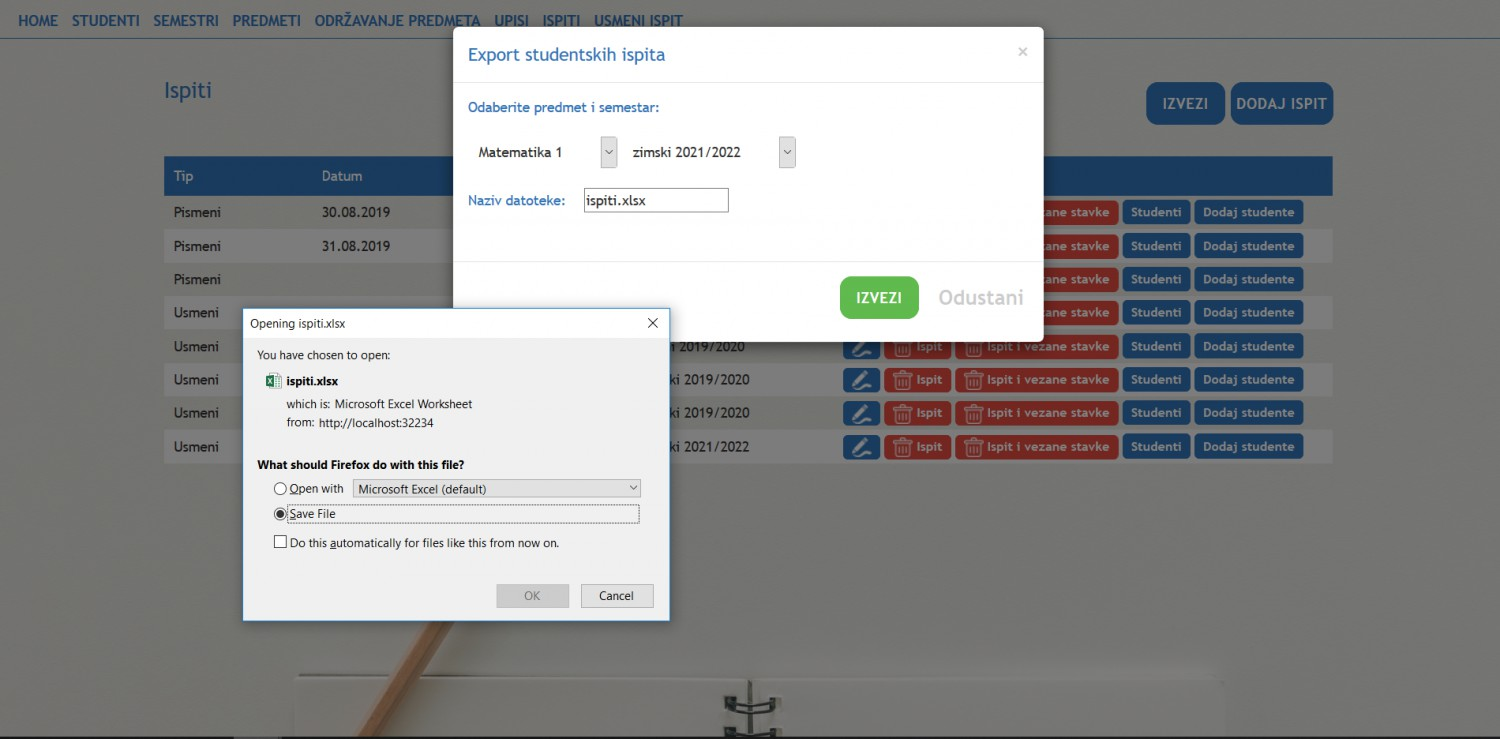
\includegraphics[width=14cm]{export.jpg}
\caption{Stranica ispiti s prikazom forme za izvoz excel datoteke}
\label{fig:export}
\end{figure}

\subsubsection{Usmeni ispit}
Za pokretanje usmenog ispita potrebno je najprije ispuniti formu (slika \ref{fig:usmeni_forma}) ili ako je na stranici ispiti kreiran usmeni ispit i dodijeljeni su mu studenti tada je putem linka moguće pristupiti usmenom ispitu.

\begin{figure}[htb]
\centering
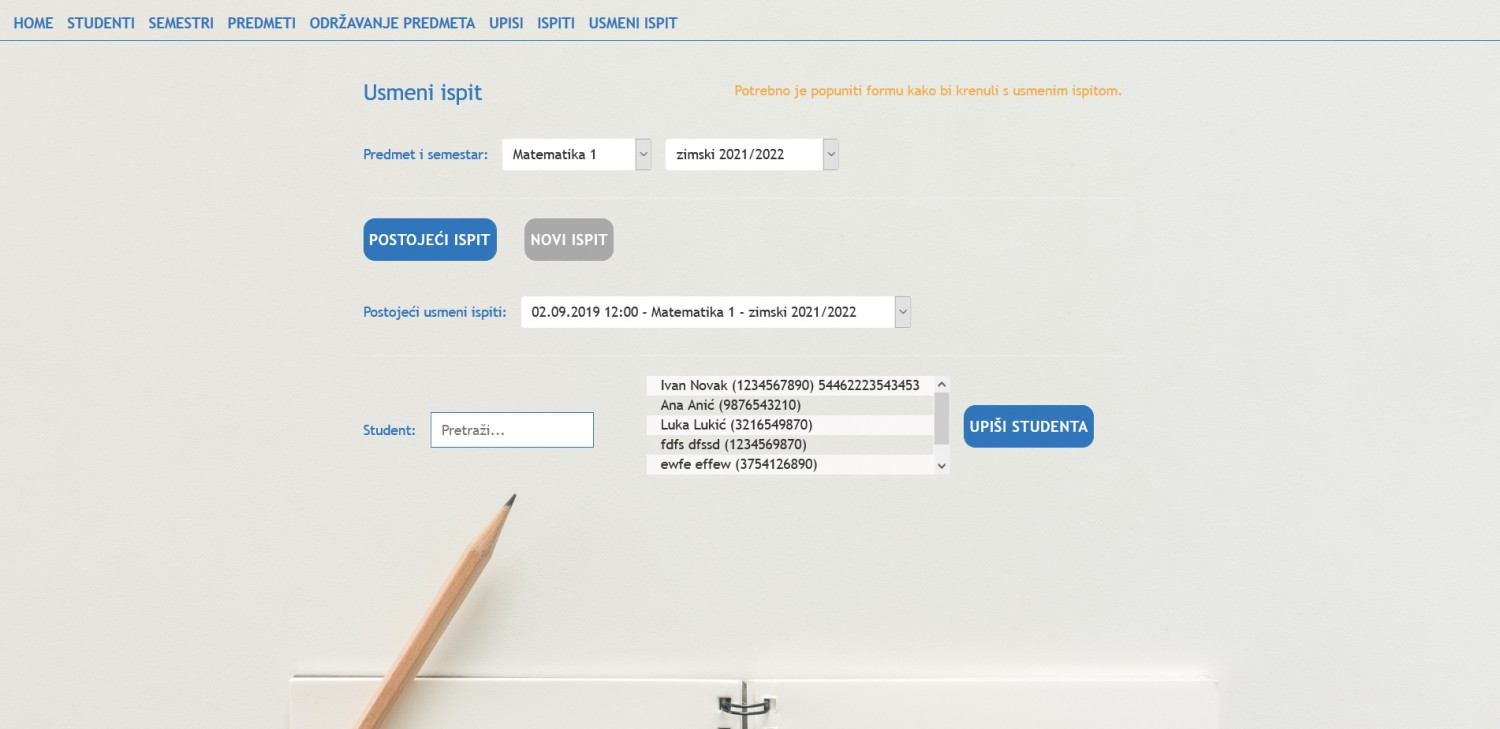
\includegraphics[width=14cm]{usmeni_before.jpg}
\caption{Forma za pokretanje usmenog ispita}
\label{fig:usmeni_forma}
\end{figure}

Forma za kreiranje usmenog ispita sadrži izbornike za predmet i semestar. Za odabranu kombinaciju dohvaćaju se postojeći usmeni ispiti. Ako se odabrani predmet ne održava u odabranom semestru ili nema postojećih usmenih ispita tada je potrebno kreirati novi ispit unosom datuma ispita. Također ako postojeći odabrani ispit nema definirani datum tada je isto prije nastavka obavezno definirati datum ili će sustav postaviti trenutno vrijeme.

\begin{figure}[htb]
\centering
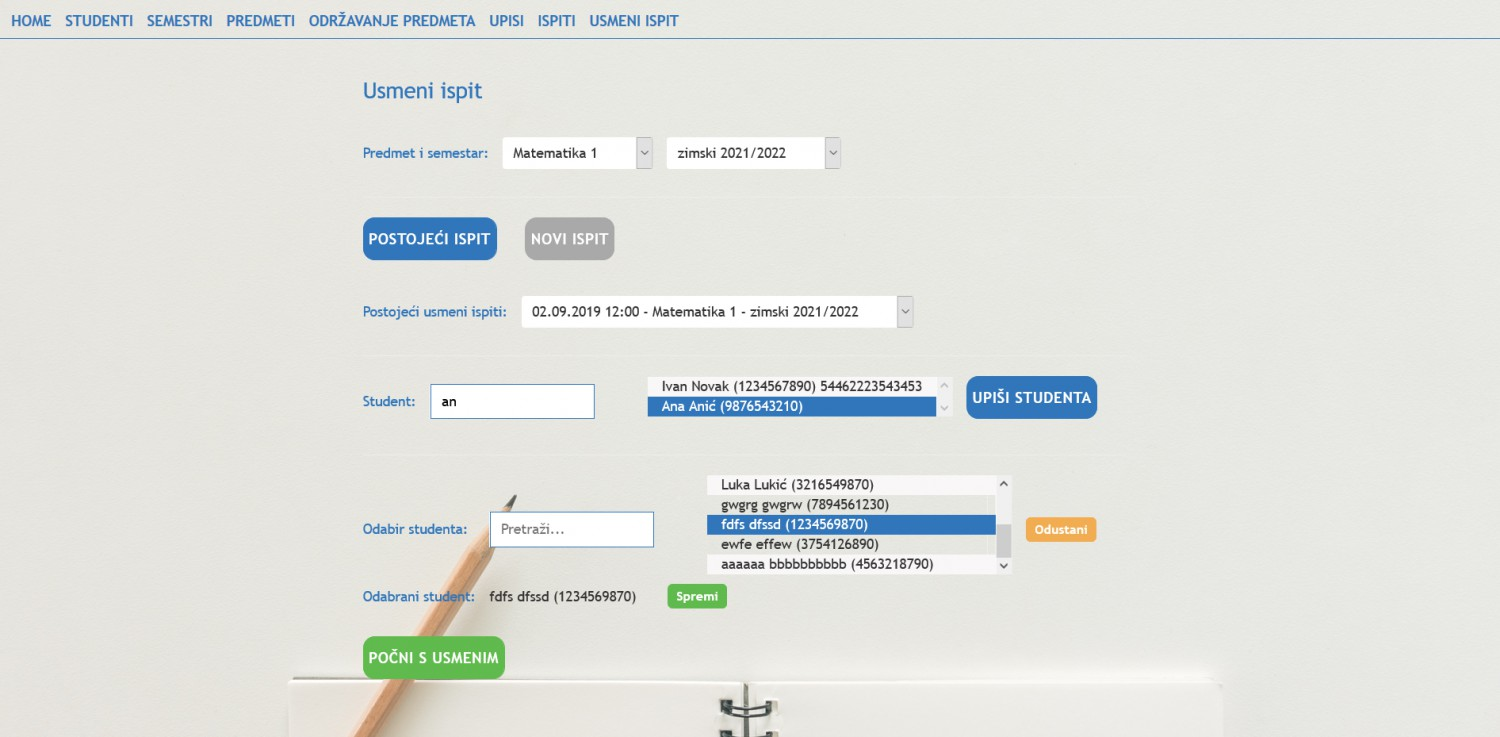
\includegraphics[width=14cm]{usmeni_after_upisistudenta.jpg}
\caption{Forma za pokretanje usmenog ispita s različitim opcijama}
\label{fig:usmeni_forma2}
\end{figure}


Nakon odabira odnosno kreiranja ispita, potrebno je odabrati studenta koji pristupa usmenom ispitu. Lista dohvaćenih studenata odnosi se na one upisane na definirani predmet u odabranom semestru. Listu je moguće pretraživati upisom u polje "Pretraži.." koje će filtrirati popis studenata. 



Ako na odabranom predmetu u odabranom semestru nema upisanih studenata ili nema određenog studenta, tada je pritiskom na gumb "UPIŠI" moguće naknadno upisati studenta. Nakon akcije upiši prikazuje se forma s listom svih studenata koje također moguće pretraživati upisom vrijednosti, te odabirom studenta i pritiskom na akciju spremi, odabrani student se upisuje na definirati predmet i semestar.

Opisane opcije unosa i pretraživanja nalaze se na slici \ref{fig:usmeni_forma2};

Akcija pokretanja usmenog ispita moguća je tek kada su odabrati predmet, semestar i student.

Nakon što je uspješno pokrenut (ili nastavljen) usmeni prikazuje se stranica s popisom osnovnih podataka o studentu, popisom osnovnih podataka o ispitu i lista svih aktivnosti studenta do sad na trenutnom predmetu.

Uz prikaz podataka postoji forma za unos pitanja ili teksta s usmenog, unos ocjene i bodova na ispitu, unos zaključne ocjene, te postavljanje zastavice da li je student pristupio tom ispitu. (slika \ref{fig:usmeni_usmeni})

\begin{figure}[htb]
\centering
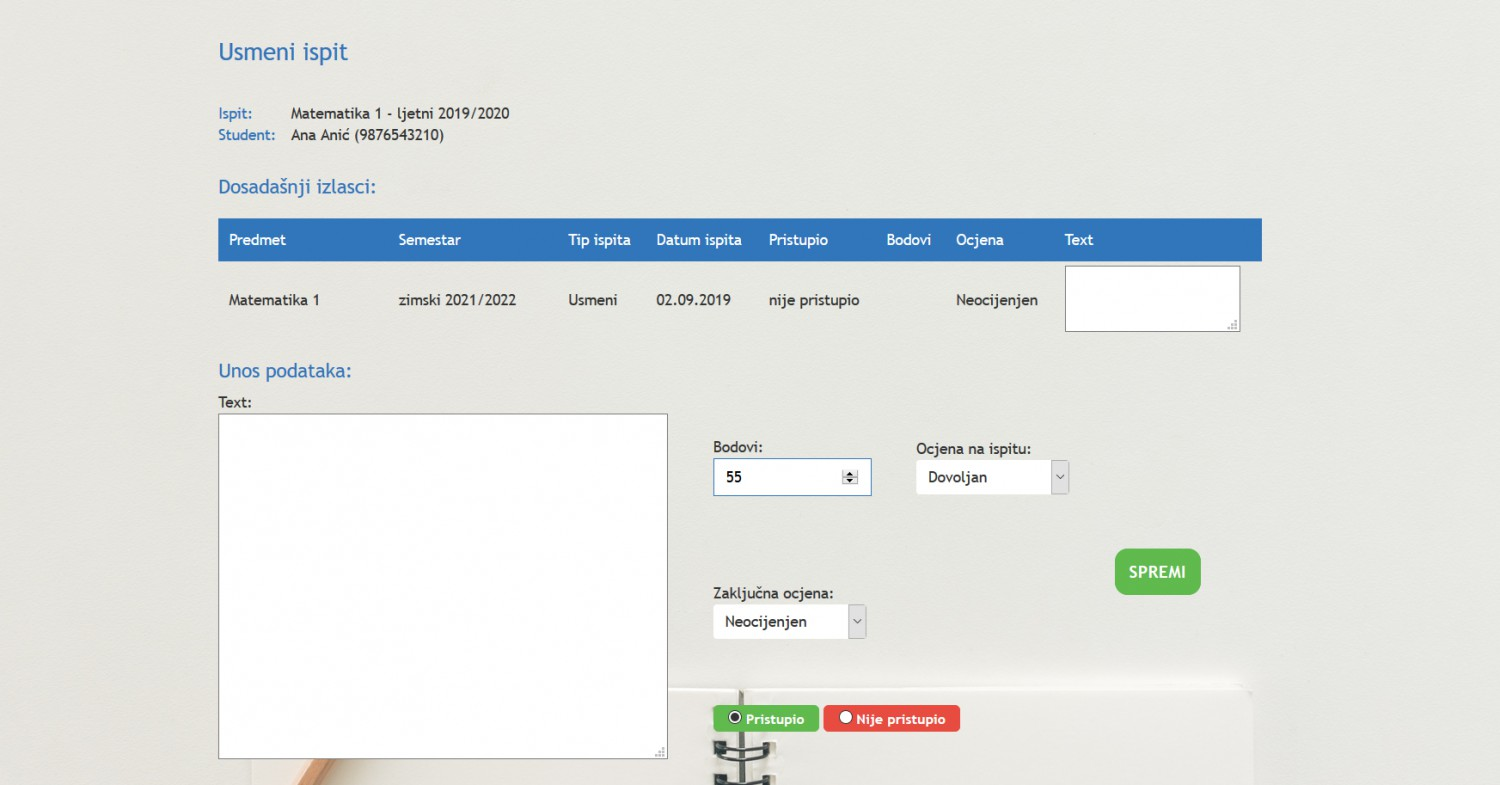
\includegraphics[width=14cm]{usmeni_usmeni_examsbefore.jpg}
\caption{Forma usmenog ispita}
\label{fig:usmeni_usmeni}
\end{figure}

\section{Windows aplikacija}
\subsection{Manipulacija osnovnim podacima}

\subsubsection{Predmeti}
Tablični prikaz osnovnih podataka o predmetima, uz mogućnost prikaza održavanja predmeta po semestrima pritiskom na gumb "Detalji" (slika \ref{fig:courses}). U sklopu prikaza predmeta dostupne akcije su uređivanje pojedinog predmeta na mjestu, brisanje i kreiranje novog. Opisani način brisanja predmeta u web dijelu primjenjuje se i ovdje jer se poziva ista metoda iz sloja poslovne logike.  
\begin{figure}[htb]
\centering
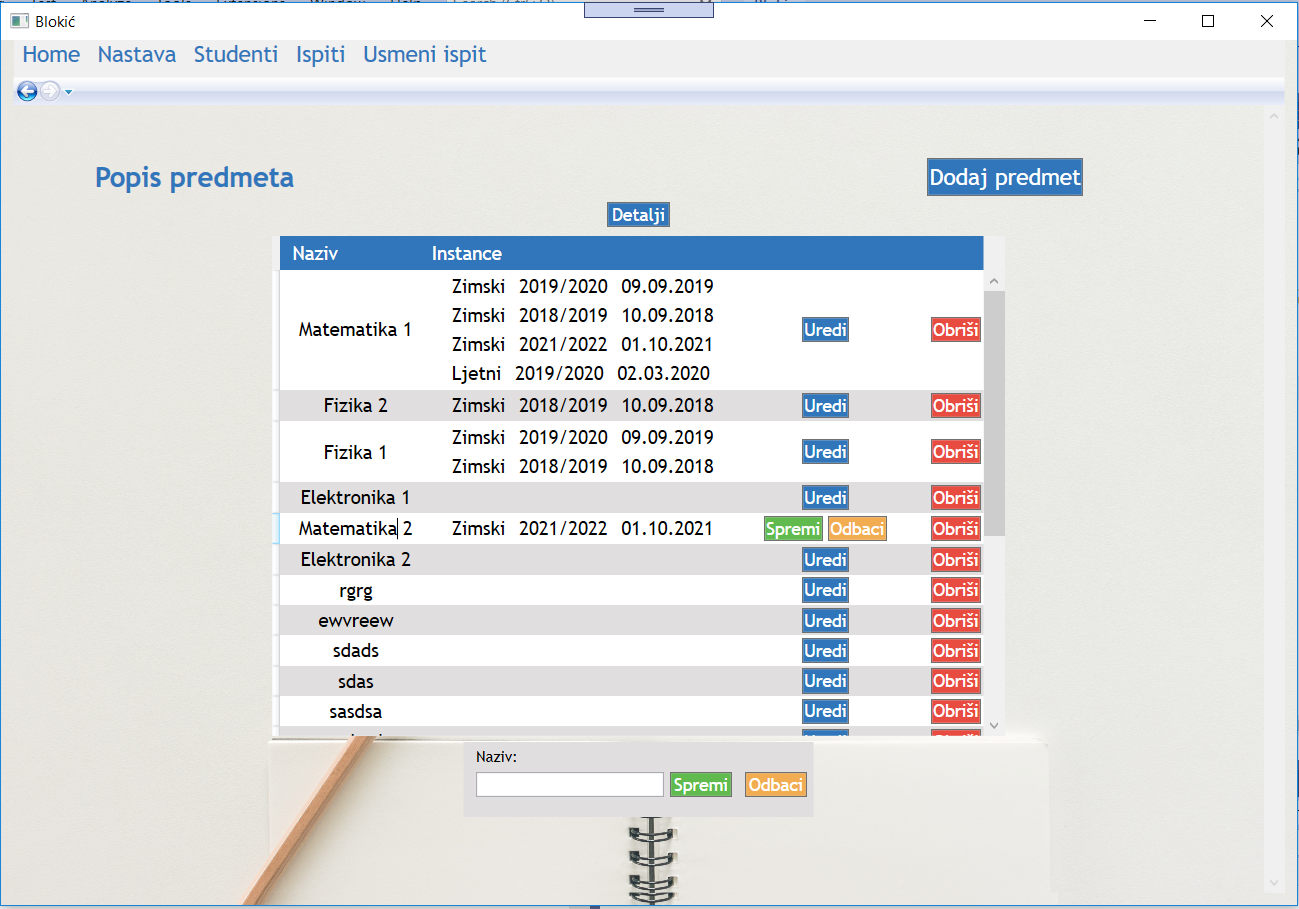
\includegraphics[width=12cm]{courses.PNG}
\caption{Stranica Windows aplikacije za prikaz, uređivanje i brisanje predmeta}
\label{fig:courses}
\end{figure}

\subsubsection{Semestri}

\begin{figure}[htb]
\centering
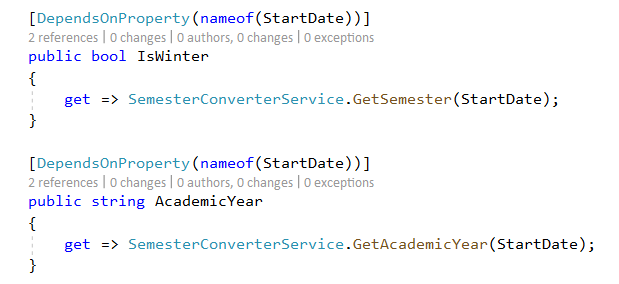
\includegraphics[width=12cm]{semester_depends.PNG}
\caption{Programski isječak u kojem se definira povezanost svojstava klase}
\label{fig:semester_depends}
\end{figure}

Popis postojećih semestara uz mogućnost promjene datuma početka i kraja ili brisanje semestra (slika \ref{fig:semesters}). Akcija kreiranja novog semestra otvara formu za unos datuma početka i opcionalno datuma završetka. Za određivanje akademske godine i vrste semestra koristi se ista metoda iz poslovnog sloja opisana u poglavlju \ref{semestri_section}.

\begin{figure}[htb]
\centering
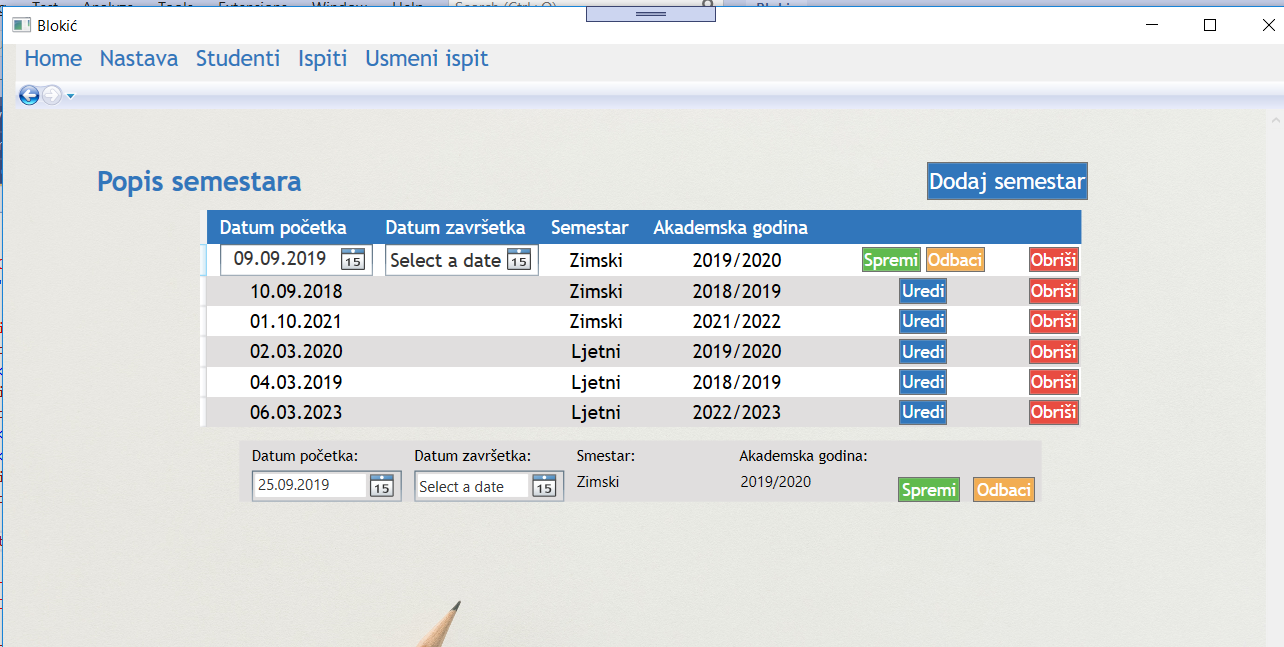
\includegraphics[width=12cm]{semesters.PNG}
\caption{Stranica Windows aplikacije za prikaz, uređivanje i brisanje semestara}
\label{fig:semesters}
\end{figure}

Poziv metode obavlja se u pozadini zahvaljujući povezanosti svojstava \engl{data-binding}. Definirana je ovisnost vrste semestra i akademska godine preko vlastitog atributa "DependsOnProperty" (slika \ref{fig:semester_depends}) o svojstvu datum početka. Kada se promjeni vrijednost datuma na Pogledu tada se pokrene događaj koji će obavijestiti Prezentacijski pogled o promjeni, koji će zatim obaviti definirane akcije. Jedna od akcija je dohvat vezanih svojstava i osvježavanje njihovih vrijednosti (programski isječak prikazan na slici \ref{fig:notifychange}).

\begin{figure}[htb]
\centering
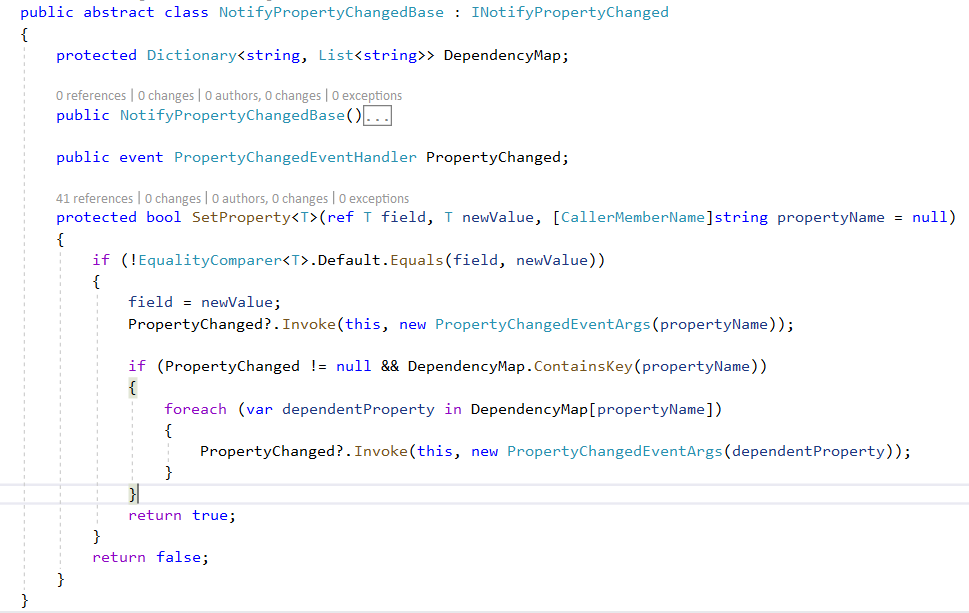
\includegraphics[width=14cm]{notifypropertychangebase.PNG}
\caption{Programski isječak u kojem se definiraju akcije koje se obavaljaju nakon promjene svojstava nad definiranom klasom}
\label{fig:notifychange}
\end{figure}

\subsubsection{Studenti}
Tablični prikaz osnovnih podataka o studentima (slika \ref{fig:studentss}). Podatke je moguće urediti na mjestu. Dostupne su akcije brisanja i kreiranja novog studenta. Kod kreiranja obavezno je unijeti ime, prezime i JMBAG. Pogreške kod unosa prikazuju se na uočljivom mjestu na vrhu stranice.

\begin{figure}[htb]
\centering
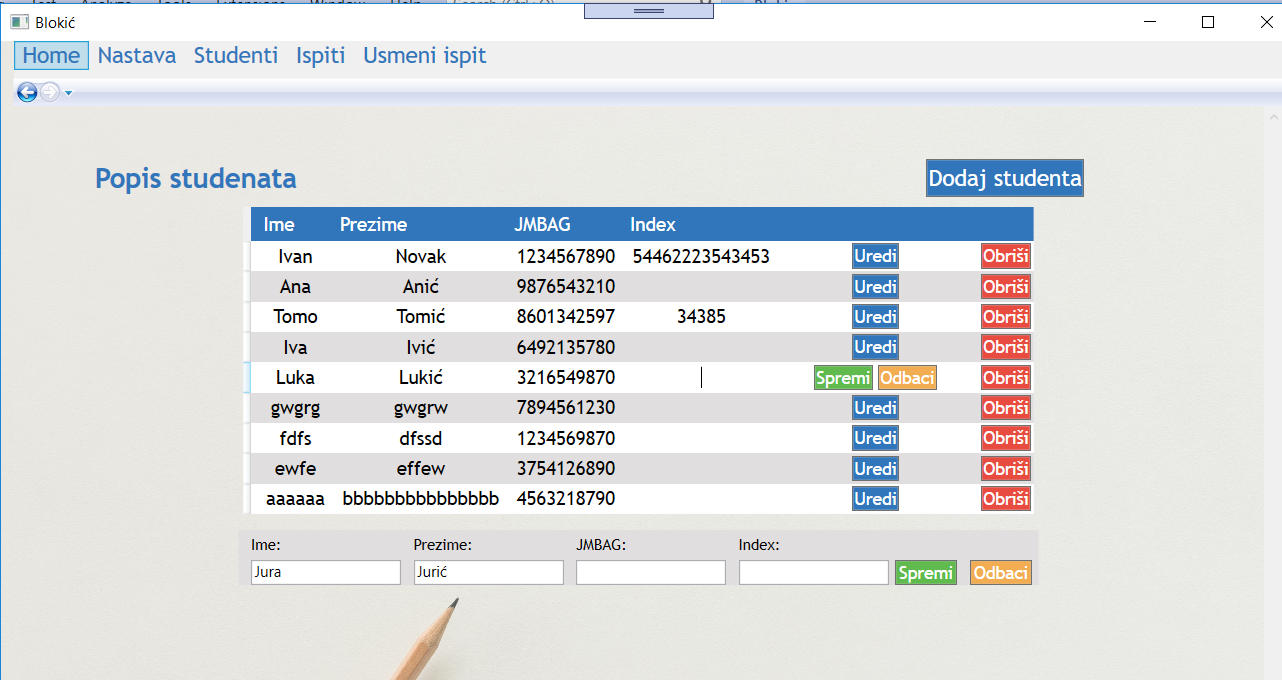
\includegraphics[width=12cm]{students.PNG}
\caption{Stranica Windows aplikacije za prikaz, uređivanje i brisanje studenata}
\label{fig:studentss}
\end{figure}

\subsection{Studentska kartica}
Dodatna funkcionalnost je takozvani prikaz kartice studenta, a sadrži sva prisustvovanja studenta na ispitima te rezultate s istih. Grupiranje i prikaz podataka jednak je kao kod web aplikacije; najprije po predmetima, a zatim po semestrima.
\begin{figure}[htb]
\centering
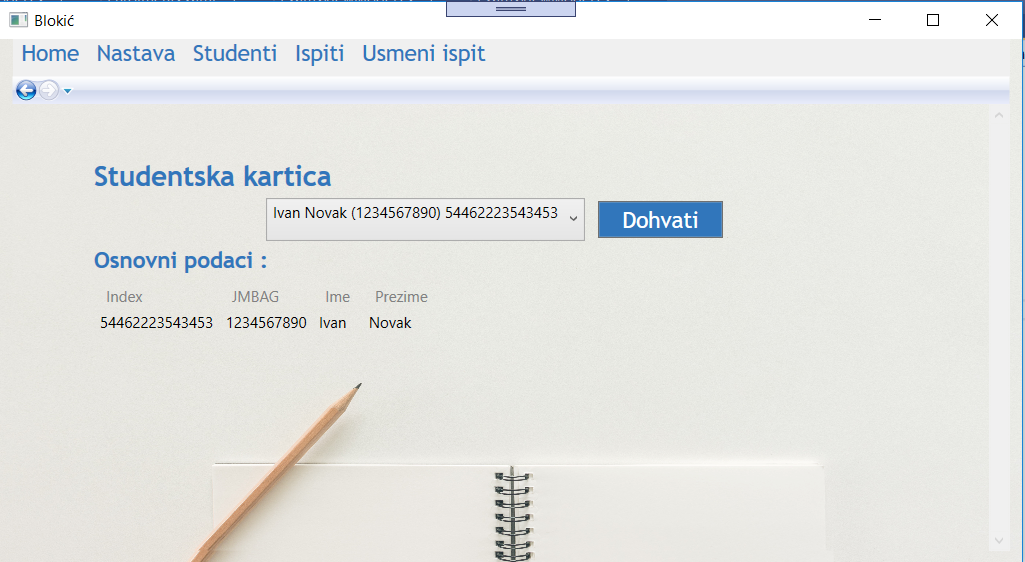
\includegraphics[width=12cm]{studentcard.PNG}
\caption{Stranica Windows aplikacije za prikaz, uređivanje i brisanje studenata}
\label{fig:studentCard}
\end{figure}

Podaci se prikazuju na novoj stranici, tako da se najprije odabere student iz padajućeg izbornika. (slika \ref{fig:studentCard})


\subsection{Održavanje predmeta i upisi studenata}

\subsubsection{Održavanje predmeta}
\begin{figure}[htb]
\centering
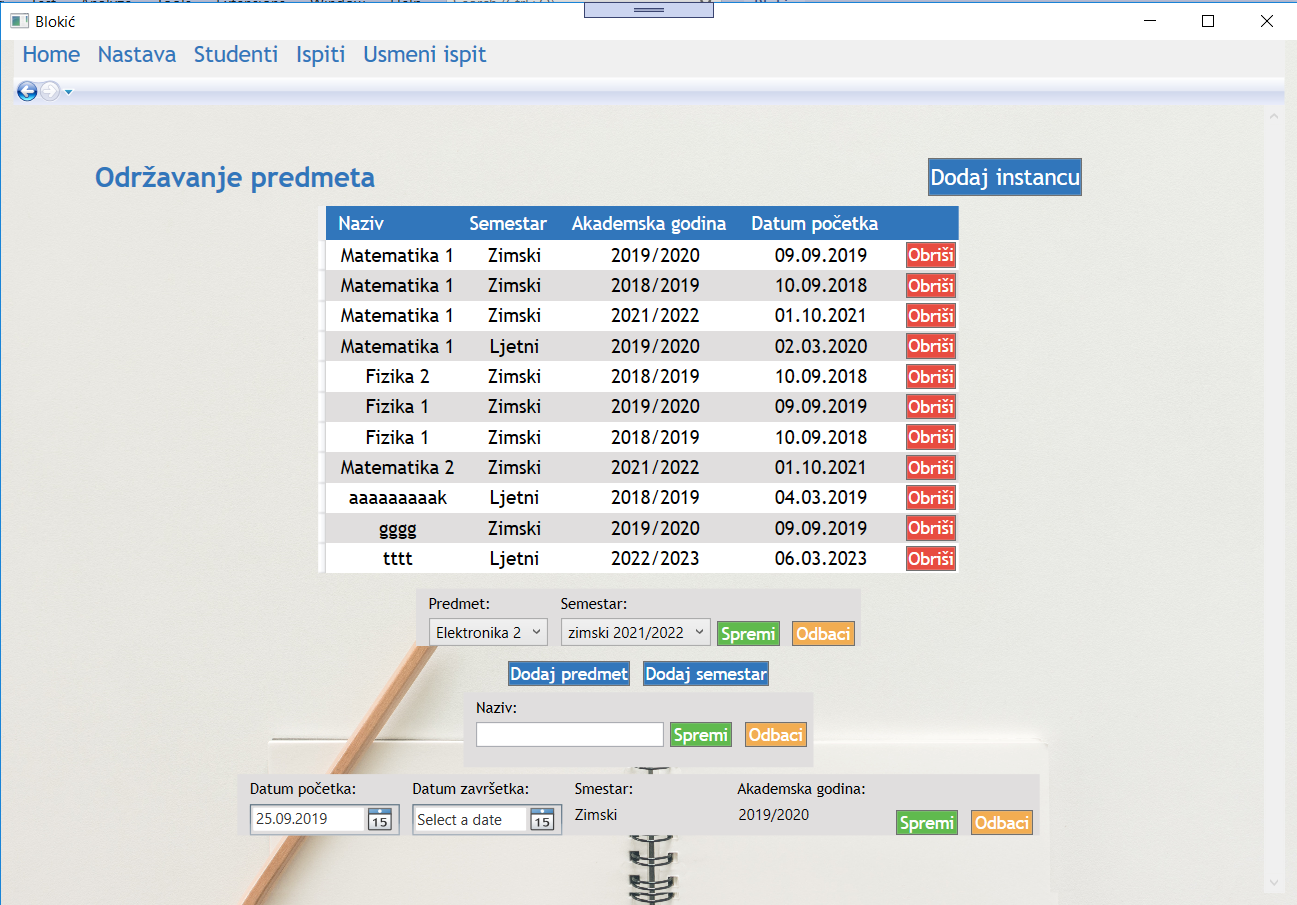
\includegraphics[width=12cm]{courseInstances.PNG}
\caption{Stranica Windows aplikacije za prikaz, kreiranje i brisanje održavanja predmeta}
\label{fig:courses}
\end{figure}

Održavanje predmeta ili instanca predmeta sastoji se od predmeta i semestra u kojem se održava bez dodatnih podataka. U samoj aplikaciji ona je glavni element koji definira sve složenije elemente. Primjerice upis studenata obavlja se na pojedinu instancu predmeta ne na sam predmet. Ispiti se također definiraju za instancu predmeta.

Stranica prikazuje popis svih kreiranih instanci uz mogućnost brisanja istih. Prikaz stranice na slici \ref{fig:courses}.

Akcija kreiranja nove instance otvara formu koja omogućava izbor postojećih predmeta i semestara ili kreiranje novih. Novo kreirani predmeti odnosno semestri, spremaju se u bazu po odabiru akcije spremi i zatim se dodaju u padajuće izbornike kako bi se mogli odmah koristiti za kreiranje instance. Zbog korištenja vezanja podataka, stranicu nije potrebno ponovno učitati već se sustav u pozadini (putem događaja \engl{events}) pobrine da se nastale promjene u podacima osvježe i prikažu na Pogledu.

\subsubsection{Upisi studenata}
Kao što je već rečeno upis studenta označava jednog studenta na jednom predmetu u jednom semestru. Kako se ocjene zaključuju na razini semestra ovaj entitet shodno tome sadrži podatke o zaključnoj ocjeni i datumu zaključivanja iste.

\begin{figure}[htb]
\centering
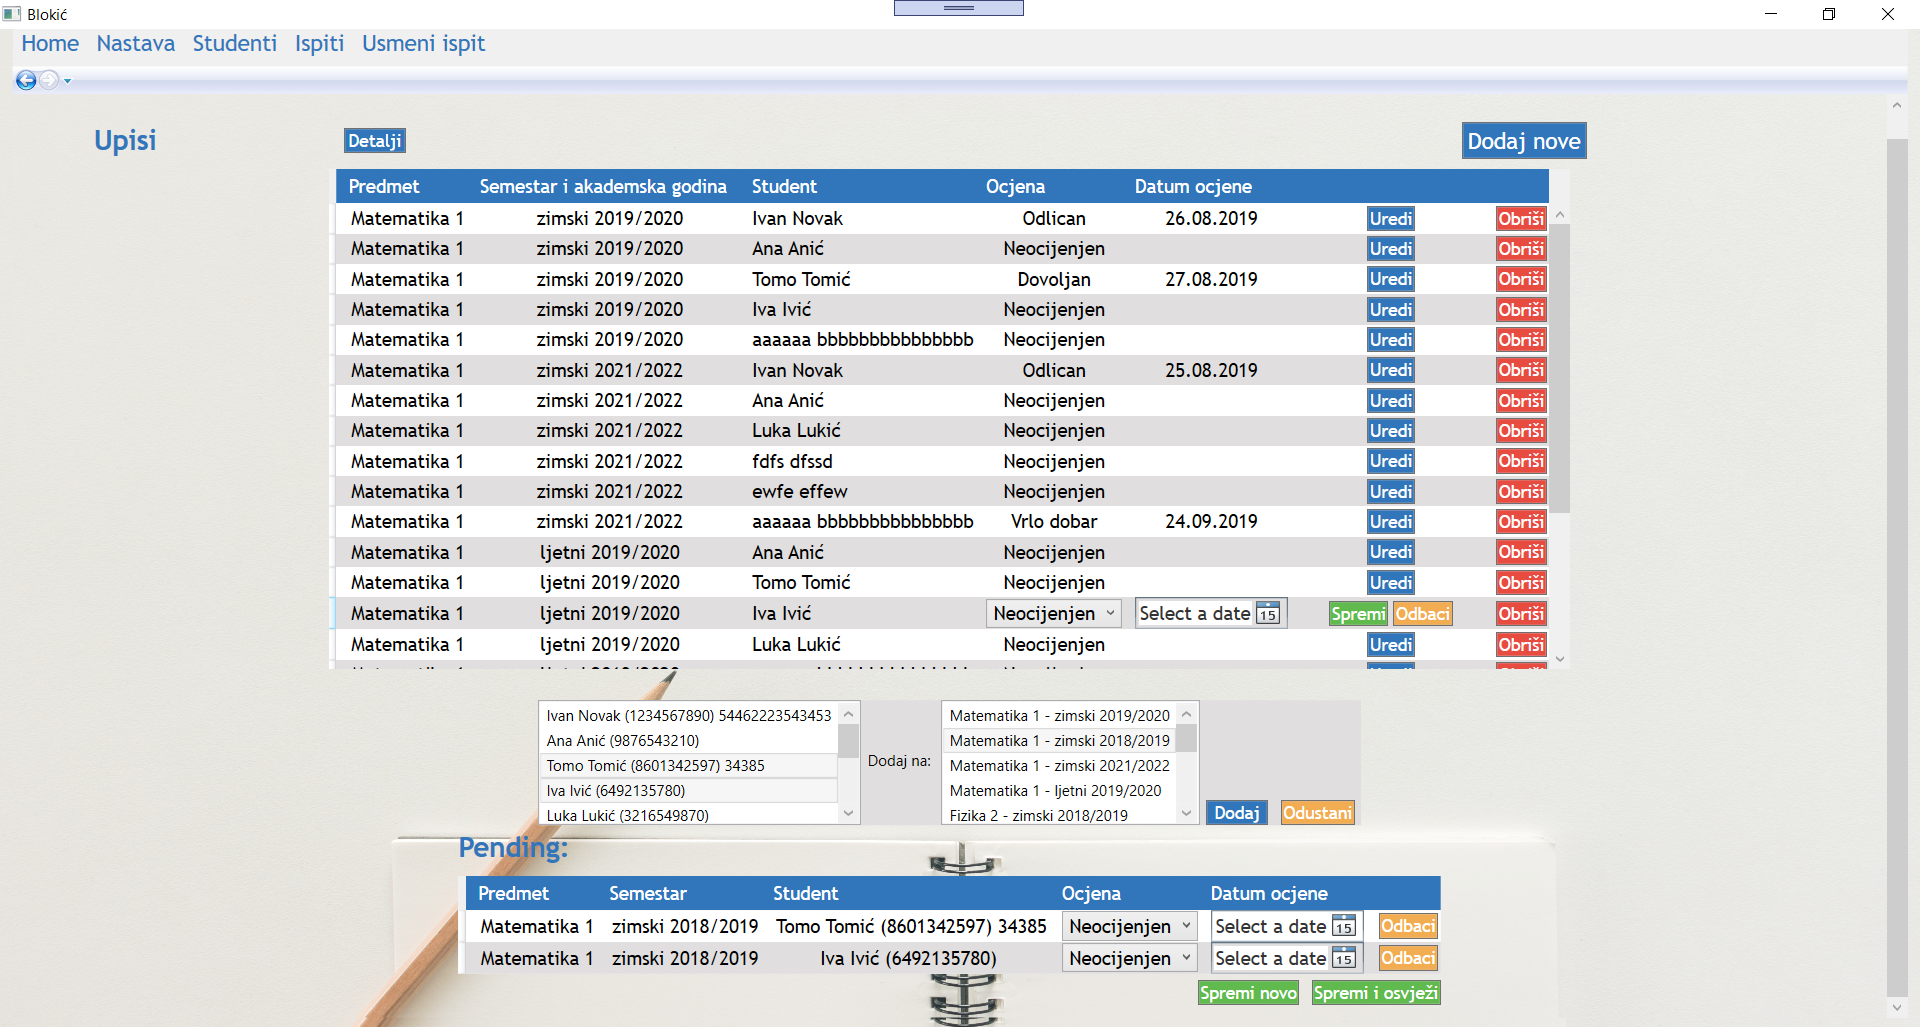
\includegraphics[width=12cm]{enrolments.PNG}
\caption{Stranica Windows aplikacije za prikaz, uređivanje, kreiranje i brisanje upisa studenata}
\label{fig:enrolments}
\end{figure}

Upisi su prikazani tablično uz mogućnost uređivanja podataka o ocjeni i datumu. Svaki od upisa također je moguće i obrisati. Prikaz stranice nalazi se na slici \ref{fig:enrolments};

Dodatna funkcionalnost prikaza i sakrivanja detalja o studentima jednaka je onoj opisanoj u web dijelu.

Akcija "DODAJ NOVE" otvara formu koja sadrži popis studenata i popis instanci predmeta. Iz obje liste moguće je odabrati nekoliko elemenata. Pritiskom na gumb "DODAJ" stvaraju se sve kombinacije odabranih elemenata iz dviju ponuđenih lista. Nastale jedinstvene kombinacije se prikazuju u listi na dnu stranice, gdje je dodatno moguće urediti podatke ili odbaciti neki od elemenata. 

Kako bi se spremili novo nastali upisi potrebno je odabrati jednu od akcija spremanja. Funkcionalnost pojedine akcije spremanja jednaka je onoj opisanoj u web dijelu.

\subsection{Ispiti}
\subsubsection{Popis svih ispita}
Stranica ispiti (slika \ref{fig:examlist}) sadrži popis svih ispita. Moguće je urediti podatke o datumu i vremenu održavanja ispita ili obrisati sam ispit. Brisanjem ispita brišu se i svi vezani podaci, što se odnosi na prisustvovanja i rezultate studenata na dotičnom ispitu.

\begin{figure}[htb]
\centering
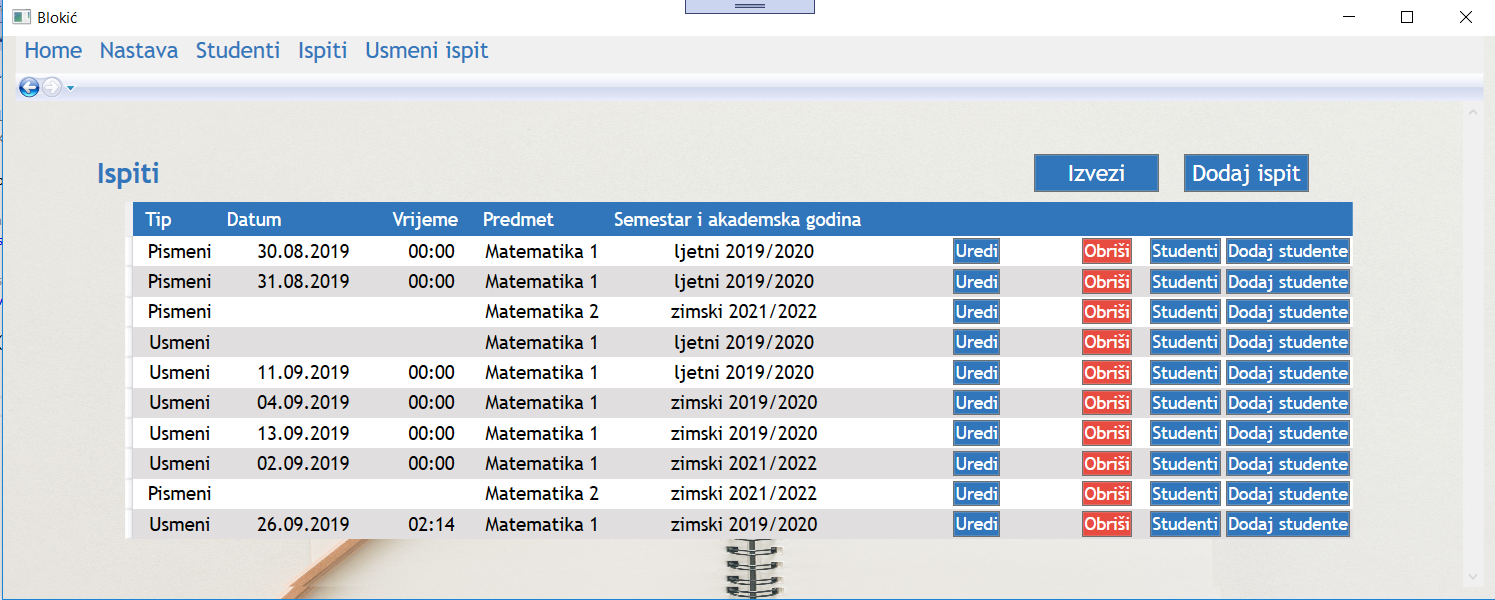
\includegraphics[width=12cm]{examlist2.PNG}
\caption{Stranica Windows aplikacije za prikaz, uređivanje, kreiranje i brisanje ispita}
\label{fig:examlist}
\end{figure}

Kod odabira akcije "DODAJ ISPIT" otvara se forma gdje je potrebno odabrati vrstu ispita i instancu predmeta. Opcionalno je moguće unijeti datum i vrijeme održavanja te odabrati studente upisane na odabranu instancu predmeta koji će pristupiti ispitu.

Dodatne akcije na stranici su :


\hfill\break
\textbf{"Studenti"} \hfill\break
Akcija obavlja dohvat i prikaz studenata koji su prijavili odnosno pristupili ispitu. Studenti se prikazuju tablično na dnu stranice te se omogućava uređivanje podataka o ispitu studenta, poput ocjene ili bodova i brisanje istih.

\begin{figure}[htb]
\centering
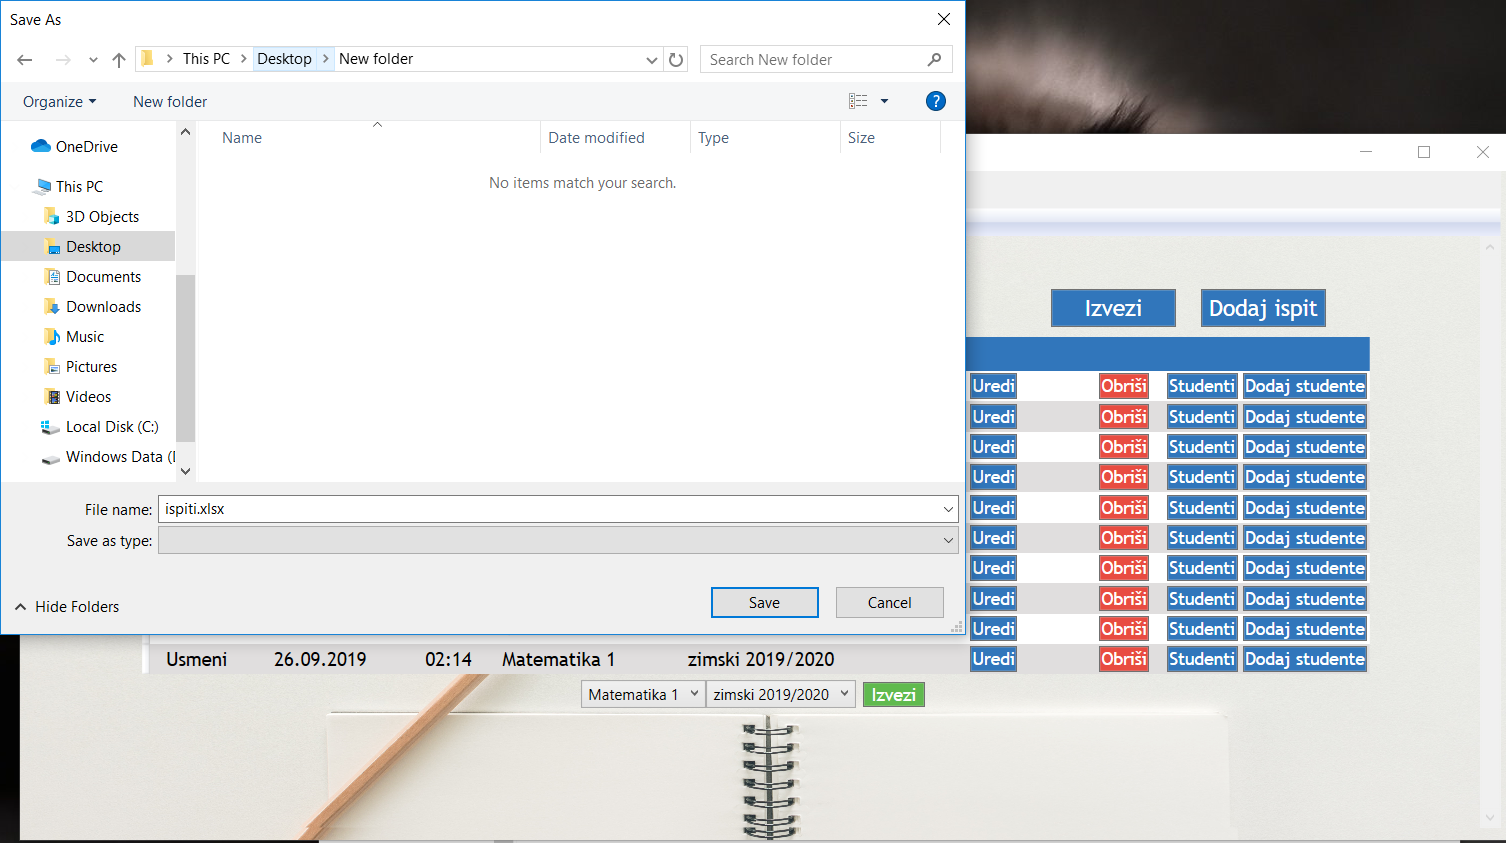
\includegraphics[width=12cm]{export.PNG}
\caption{Stranica Windows aplikacije kod izvoza excel datoteke}
\label{fig:exportDesktop}
\end{figure}


\hfill\break
\textbf{"Dodaj studente"} \hfill\break
Akcija prikazuje formu gdje je moguće odabrati studente upisane na instancu predmeta za koju je ispit definiran, koji će se zatim prijaviti na taj ispit.

\hfill\break
\textbf{"Izvezi"} \hfill\break
Akcija prikazuje formu u kojoj je potrebno odabrati predmet i semestar za koji će se kreirati izvještaj o ispitima i studentskim rezultatima. Temeljem odabira kreira se izvoz podataka u Microsof Excel datoteku. Nastala datoteka je jednaka neovisno o aplikaciji iz koje se zatraži izvoz zato što se poziva isti servis iz poslovnog sloja. Forma za unos i prozor za spremanje datoteke prikazani na slici \ref{fig:exportDesktop}.



\subsubsection{Usmeni ispit}
\begin{figure}[htb]
\centering
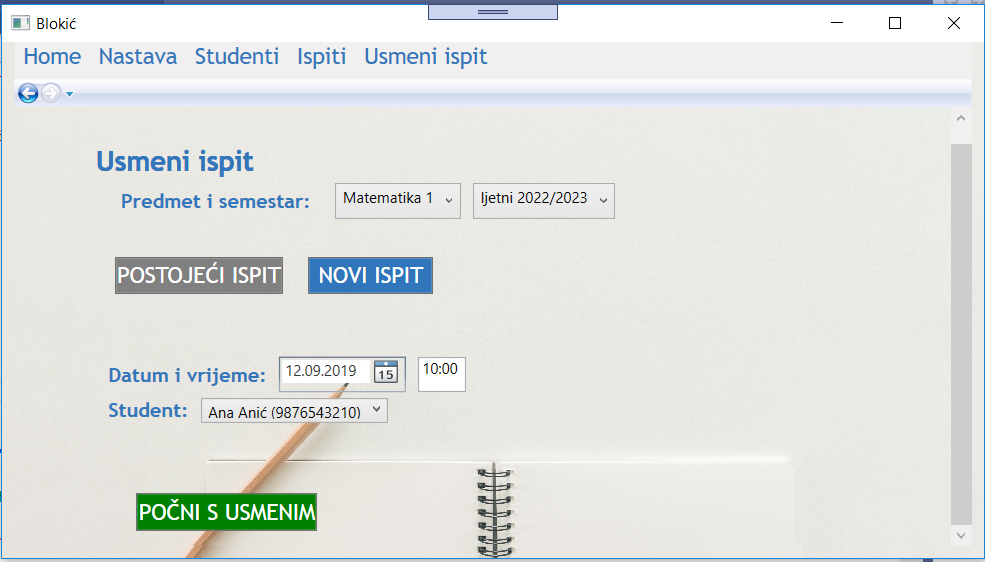
\includegraphics[width=12cm]{oral.PNG}
\caption{Stranica Windows aplikacije za unos forme kod pokretanja usmenog ispita}
\label{fig:oral}
\end{figure}


Napredna funkcija sustava je obavljanje usmenog ispita. Kako bi se pokrenuo usmeni ispit potrebno je popuniti formu (slika \ref{fig:oral}) koja će kreirati ili dohvatiti postojeći usmeni ispit za odabranog studenta. Osim studenta u formi je potrebno odabrati predmet i semestar, ovisno o njima se zatim odabire postojeći ili se kreira novi usmeni ispit.


\begin{figure}[htb]
\centering
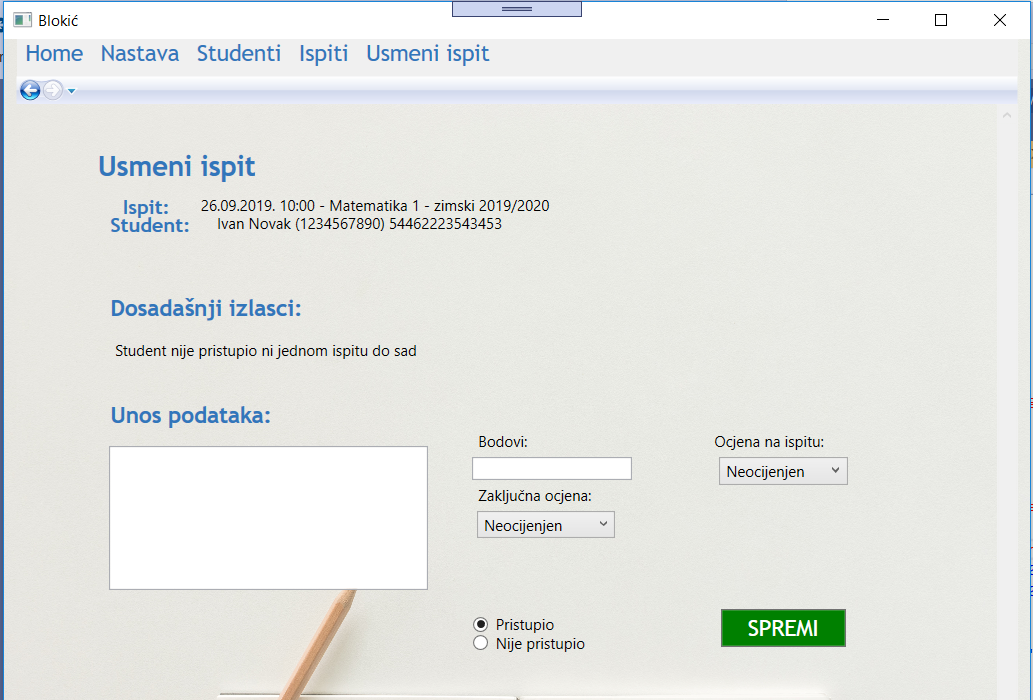
\includegraphics[width=12cm]{oral2.PNG}
\caption{Stranica Windows aplikacije za unos podataka iz usmenog ispita}
\label{fig:oral2}
\end{figure}

Nakon što su ispravno popunjeni podaci u formi moguće je pokrenuti ispit. Pokretanjem ispita prikazuju se podaci o studentu i forma za unos podataka iz usmenog ispita (slika \ref{fig:oral2}).


Podaci o studentu sadrže osnovne identifikacijske podatke i tablicu s prikazom dosadašnjih izlazaka i rezultata studenta iz ispita na trenutnom predmetu.


Forma za unos podataka iz usmenog ispita sadrži polje za unos pitanja, unos bodova i odabir ocjene te unos zaključne ocjene.

%\chapter{Korištenje aplikacije}

\chapter{Zaključak}
Cilj izrade rada bio je proučiti podršku obrasca MVVM u programskom okviru .NET Core kroz izradu dviju aplikacija (web-aplikacije i Windows-aplikacije). U svrhu  proučavanja podrške odabrana je tema nastavničke evidencije studenata na pismenim i usmenim provjerama. Programsko rješenje napravljeno je kao višeslojni sustav, gdje obje aplikacije komuniciraju sa zajedničkim poslovnim slojem koji obavlja pretvorbu poslovnih modela u modele baze uz komunikaciju sa slojem za pristup podacima. Višeslojna arhitektura sustava podržana je i u implementaciji MVVM obrasca u aplikacijama. Sam obrazac diktira odvajanje prezentacijskog sloja i prezentacijske logike od poslovnog sloja. Takvim načelom dizajna aplikacije na poslovni sloj otpada puno manje rada. Većina aplikacijske logike nalazi se u prezentacijskom modelu iz MVVM-a. Odvajanje logike omogućava lakšu nadogradnju i promjene. Opisan pristup idealan je za srednje do veće aplikacije gdje se odvajanjem programskog koda potiče brži razvoj, a sami prezentacijski modeli su relativno mali te ne uzrokuju spori rad aplikacije zbog potrebe za kontinuiranim parsiranjem i prosljeđivanjem podataka. Usporedbom dviju nastalih aplikacija uviđa se znatna konceptualna sličnost u kreiranju i postignuta modularnost sustava.

\bibliography{literatura}
\bibliographystyle{fer}

\begin{sazetak}
U okviru ovog rada istražena je podrška obrasca MVVM u programskom okviru .NET Core. Korištene su dvije vrste aplikacija; web-aplikacija i Windows-aplikacija. 
Svrha izrade aplikacija bila je evidencija rezultata studenata na pismenim i usmenim ispitima. Prema danim zahtjevima na sustav odabrane su i opisane arhitektura sustava, alati i tehnologije.
Predstavljen je pregled funkcionalnosti sustava uz prateće detalje implementacije.
Dan je opis korisničkog sučelja i način uporabe programskog rješenja.

\kljucnerijeci{web-aplikacija, Windows-aplikacija, MVVM, .NET Core, nastavnička evidencija}
\end{sazetak}

% TODO: Navedite naslov na engleskom jeziku.
\engtitle{MVVM pattern and .NET Core framework}
\begin{abstract}
This paper explores support for MVVM pattern using .NET Core framework. Two types of applications were used; web application and Windows application. Application purpose is tracking of student's results on written and oral exams. Based on the given requirements system architecture, tools and technologies were chosen and described.  
System functionality is represented with accommodating implementation details. User interface specification is provided as instructions for usage of software solution.


\keywords{web application, Windows application, MVVM, .NET Core, exam records}
\end{abstract}

\end{document}
